\documentclass[11pt]{report}
\usepackage{fullpage}
\usepackage{graphicx}
\usepackage{float}
\restylefloat{table}
\usepackage{url}
\usepackage[toc, page]{appendix}
\usepackage{listings}
\begin{document}
\title{Developing a tool for teachers to increase awareness and understanding of Autism}
\author{Ashley Peacock}
\maketitle
\tableofcontents

\chapter{Overview}

The projected started by firstly creating and considering various project proposals that may benefit people with ADHD or Autism. Following this, research and feedback aided the selection of the project an "Autism Simulator" whereby the user plays as a child with Autism and gets to experience some of the difficulties, specifically sensory related difficulties through their eyes. Consultation with the Learning and Adaptive Environment Research(LAER lab) in addition to interviews with people on the Autistic spectrum, professionals and school teachers further solidified this selection and gave indication of the challenges faced as to inform design choices and goal selection. A prototype of the simulator was created using a game engine to quicken development and the project was evaluated by the LAER group with an additional evaluation in the form of an on-line survey where participants were able to view a video demo of the simulator and give feedback. The first playable version was subsequently created after an extensive re-write and addition. A final formative evaluation was conducted with various students to aid game-play decisions and improvements before two similar evaluations were carried out; one online and one in person and was completed by various members of the university involved in education. \\

Below is a summary of the projects overall aims and goals which were further discussed and identified in \ref{goalsandrestrictions}:\\
\textbf{Questions:}\\
\begin{enumerate}
\item Develop a simulator that allows users to play as an autistic child and thereby experience some of the difficulties/obstacles faced
\item Focus on sensory difficulties but include some other information about autism.
\item Allow the user the ability to obtain useful information on how possible household items/situations can trigger sensory problems as well as how a child with autism might cope with these.
\item Increase understanding and awareness of autism and the difficulties faced.
\end{enumerate}

\section{Selecting a project}
The project started with the purpose of creating software to benefit someone with Autism, ADHD or those in contact with these conditions such as family members or carers. Both Autism and ADHD are developmental disorders that start from birth and affect the individual's attention, concentrations and ability to fit into mainstream society.

Owing this was a very broad topic with many possible avenues, multiple proposals were put forward and a selection was made following an online questionnaire, speaking to professionals and parents of children with Autism and ADHD at the ADDISS Conference(2012) and consideration of factors such as the learning curve and plausibility of each project given time constraints.

Project proposals:
\begin{table}[H]
    \begin{tabular}{| p{2cm} | p{5cm} | p{4cm}| p{6cm} |}
    \hline
    Proposal name & Description &  For & Against \\
    \hline
    \hline
    Online diary & Online system to improve communication between carers, parents, social workers, schools. Parties could post questions and ask for suggestions when dealing with certain behaviours as well as document the child's day allowing easier identification of patterns of behaviour or problems & 
   Seamless communication between doctors, teachers and carers which is problematic and information can be missed.
   & \begin{minipage}{5cm}
    \vskip 4pt
    \begin{enumerate}
   \item Good in theory but may not be practical due to data protection.
   \item Relies too heavily on parents/carers being able to read emails or notifications.
   \item May be difficult for some schools to gain access to wifi.
   \end{enumerate}
   \vskip 4pt
 \end{minipage}                        \\
    \hline
    Social simulator & Simulated social scenarios for autistic users to trial various social situations and see possible outcomes whilst being given potential tips and strategies & & \begin{minipage}{5cm}
    \vskip 4pt
    \begin{enumerate}
   \item Big project given time-frame
   \item Other companies working on similar concepts and much research has been done on this topic already.
   \end{enumerate}
   \vskip 4pt
 \end{minipage}     \\
    \hline
    Dynamic scheduler and planner app & A planner that would re-schedule tasks when not completed and present basic to-do lists with tasks broken down into manageable chunks &
    No planners available that specifically target planning/executive functioning difficulties within ADHD/Autism.
  &
Least unique proposal, many other planners available.
  \\
    \hline
    Environment app & Phone app aimed to encourage children to engage with the environment around them with simple questions and pictures: "Can you see a blue car?".  & 
    Least amount of implementation work, could be simple but effective.
 & \begin{minipage}{5cm}
    \vskip 4pt
    \begin{enumerate}
   \item Hard to back up with literature 
   \item Difficult concept to understand
   \end{enumerate}
   \vskip 4pt
 \end{minipage}    \\
    \hline
    \end{tabular}
\end{table}

\begin{table}[H]
    \begin{tabular}{| p{2cm} | p{5cm} | p{4cm}| p{6cm} |}
    \hline
    Proposal name & Description &  For & Against \\
    \hline
    \hline
   Autism simulator & A 3D virtual environment where the user plays as a child with autism and can thus experience some of the obstacles faced through a visual/game environment & 
   \begin{minipage}{4cm}
    \vskip 4pt
    \begin{enumerate}
   \item Most unique and popular idea
   \item Misunderstanding from public is a big problem
   \item Could be extremely helpful in aspects such as teacher's training which is expensive.
   \end{enumerate}
   \vskip 4pt
 \end{minipage}   &
 \begin{minipage}{5cm}
    \vskip 4pt
    \begin{enumerate}
   \item Big project given the time frame, no previous simulators at the time of selection that could be drawn from.
   \item  No evidence or backing from literature available
   \end{enumerate}
   \vskip 4pt
 \end{minipage}    \\
    \hline
    \end{tabular}
\end{table}

The planner was eliminated on the basis of being the least unique concept with many currently available. Descriptions of the four remaining projects were put on a website and people were asked to complete a questionnaire with their preferences. Participants were asked to rank 1-3 which proposals they felt would be the most beneficial to the community as well as answering the following quantitative questions: 

\begin{enumerate}
\item Please give some information about yourself, for example if you have ASD/ADHD or are a professional/carer.
\item Please select and rank three proposals you feel are the best
\item Please explain reasons for selection
\end{enumerate}

\subsection{Results}
It was completed anonymously by five people in total and included people with ASD/ADHD, professionals, carers and parents:

\begin{table}[H]
    \begin{tabular}{| p{2cm} | p{3cm} | p{3cm}| p{3cm} | p{4cm} |}
    \hline
    No. & Rank 1 & Rank 2 & Rank 3 & Comments on candidate \\ \hline
    1 & Autism Simulator & Social Simulator & Diary & PHD student and project supervisor for informatics UG4 projects at Edinburgh University\\ \hline
    2 & Autism Simulator & Diary & Social simulator & Parent of two children with ASD/ADHD. Works professionally with young people with disabilities and their carers\\ \hline
    3 & Social Simulator & Autism Simulator & Diary & Parent of two children with ASD\\ \hline
    4 & Autism Simulator & Social Simulator & Environment app & Adult with Autism. \\ \hline
    5 & Social simulator & Autism simulator & Diary & Not specified \\ \hline
    \end{tabular}
\end{table}

Participants 1 and 2 gave individual written feedback on each project as well as completing the survey. In addition, one person chose to give feedback on the individual projects rather than filling out the questionnaire. This person is a professional and counsellor to neurodiverse adults and has setup support groups and workshops for many years. 

Comments on the individual projects can be summarised below:

\begin{table}[H]
    \begin{tabular}{| p{3cm} | p{12cm} |}
    \hline
    Project name & Comments \\ \hline
    Autism Simulator & Most highly thought of concept. Worries about the concept being far too big. A book called "skallagrigg" which a person with cerebral palsy creates a similar game and was the topic of an AS reading group. People in the group said that they would love for such a thing to exist\\ \hline
    Environment app & Generally quite difficult to back up with literature. Concept was generally difficult to understand and not well explained on the website. However, commented that as children with autism tend to love technology/ipads it could provide a motivator to access the world and help deal with overwhelming stimuli\\ \hline
    Social simulator & Social situations are too unpredictable and hence social simulations tend to be catered for the individuals however, giving strategies and suggestions could work quite well. There's also lots of others working on these concepts and it already had a large base of literature demonstrating the challenge to the task. \\ \hline
    Diary & Data protection could be an issue. Limited use of Wifi and computers in school could make it inaccessible. In a play-scheme context it is a good idea in theory, but again getting use of a computer would be difficult. A phone/text system might work better. People also tend to include opinions and perspectives of situations and this may present additional problems. \\ \hline
    \end{tabular}
\end{table}

\subsection{Conclusions}
From the results of the questionnaire it became obvious which of the three concepts people felt were the most beneficial although the Environment app's score may have suffered due to not being particularly well explained. One of the key goals for this project is to create and artefact that can be used within the community and as such the "Diary" was eliminated on the basis of data protection and confidentiality problems. This left two projects the autism and social simulator. The autism simulator was selected as from all sources, responses were the most positive with the only concern being its potential size and lack of restriction, which could be eliminated by conveying a subset of autistic difficulties and if a game engine was selected for development rather than creating the graphics engine from scratch it should alleviate any concerns of the time restraints. The first limitation from the outset was to restrict the simulator to a home environment and this selection will be discussed in slightly more detail. 

\chapter{Literature review}

\section{What is Autism?}

Autism is a life-long condition which affects how an individual may perceive and communicate to the world around them\cite{nas}. It is currently diagnosed by the presence of atypicalities in two domains: Restricted and Repetitive Behaviours(RRBs) and Social communication.

Firstly RRBs which entail insistence on sameness(IS) such as keeping strict routines and can come with distress with small changes, repetitive movements, flipping objects or echolalia and in addition encompasses sensory atypicalities \cite{dsm52}. These can lead to challenging behaviours defined as self-injurious, aggressive, inattention or disruptive behaviours\cite{teacherchallenge}, however the National Autistic Society suggested these behaviours are not stopped as they may serve unknown function,
 
The second domain is social communication and interaction deficits; an individual with autism may struggle with non-verbal ques such as body language, facial expressions, eye contact and understanding of gestures. In addition to adjusting behaviour in social contexts, difficulty in imaginative play or making friends.  

As a spectrum disorder, the range and severity of symptoms are unique to each person and thus a person with autism is classified into three different levels with the first requiring some support and the latter requiring substantial amounts\cite{dsm52}. Those on the low-functioning level of the spectrum, may have little to no verbal language and prefer to communicate using visual mediums such as PECS. For those with autism on the high-functioning side of the spectrum(i.e Aspergers) their difficulties can be less obvious; they may develop superb language skills but have difficulty using these in a social context which may lead to unintentional social offence or ridicule. Deficits with social imagination and theory of mind create difficulty in seeing another person's perspective and can lead to miscommunication and misinterpretation. 

With some of the disadvantages that may come with having autism, there are reported strengths that arise from their unique cognitive style i.e a talent for spotting details\cite{bayes} or having an impeccable memory of facts in relation to their 'special interests'. This further gives rise to the notion that Autism is not a disability, but a cognitive difference with it's own set of positives and negatives. 

In the last decade there has appeared to be improvements in public perception and understanding of autism and other cognitive differences such as Dyslexia and ADHD but there is still much left to be desired. Figures drawn from the 2011 census estimate that 1.1\% of the population have Autism\cite{nas} and as this figure has greatly risen\cite{increasingprevalence} so too has the need for greater public awareness and understanding\cite{autism_awareness} resulting in millions of pounds being spent on campaigns across the globs, such as World Autism Awareness Day and Light it up blue organised by Autism speaks(2013)\cite{autism_awareness}. 

A survey published by the National Autistic Society revealed that 92\% of respondents had heard of Autism but only 48\% had heard of Aspergers syndrome which has less obvious difficulties. Research has indicated that general members of the public are aware of communication and social issues that come with autism\cite{autismmisconception}, but little are aware of sensory difficulties\cite{autism_awareness}. In \cite{autism_awareness}, of 1204 people surveyed, 293 were aware of communication difficulties, 131 social but only 12 were aware of sensory difficulties. These is alarming owing "Many people with Asperger syndrome/High functioning autism define their sensory processing problems as more disabling than the deficits in communication/social behaviour\cite{olgab}.

\begin{quote}
If I could make one change... every person who comes into contact with my daughter would have some form of training in autism.\cite{nasschool}
\end{quote}

\section{Sensory Experiences}
Sensory processing differences in autism are highly reported, 81\% of respondents reported differences in visual perception, 87\% in hearing, 77\% in tactile perception, 30\% in taste and 56\% in smell \cite{sensory_leisure}. Senses play a vital role in how we model and perceive the world around and differing sensory experiences can result in differing views and behaviours.
 
Senses in autism can be hyper(more sensitive), hypo(less sensitive), agnostic or fluctuate between hyper and hypo\cite{bayes}. Fluctuations can be described as a "FM radio that is not exactly tuned on the station when you are driving down the freeway. Sometimes the world comes in clearly and at other times it does not" \cite{olgab}. As with all areas of autism, sensory atypicalities are unique to each individual, however, fluctuations can create a particular challenge for the individual and for carers in being able to predict troubling sources before they occur. 

When a sensory channel is in a state of agnosia, although able to see, one may not be able to assign it to any meaning, the individual becomes 'mind-blind', or 'mind-deaf' and consequently act as if they are genuinely deaf or blind. Below are examples of the effects someone with autism may experience depending on the state of their sensory channel:

\begin{table}[H]
    \begin{tabular}{| l | p{5cm} | p{5cm} |}
    \hline
    Sense channel & Hyper                                                                                                                      & Hypo                                                                   \\
    \hline
    \hline
    Vision        & Vision may be magnified                                                                                                    & Attracted to light or fascinated with bright colors                    \\
    \hline
    Auditory      & Sounds are amplified. Temple Grandin a write with autism described her ears as like 'microphones'                          & Is attracted to sounds/noises                                          \\
    \hline
    Tactile       & Clothes may hurt. One person with autism described clothe labels as feeling like 'barbed wire'. May not like being hugged. & Enjoys being hugged or seeks pressure by crawling under heavy objects. \\
    \hline
    Taste/Smells & Smells or texture of foods may be intolerable. & Mouths and licks objects \\
    \hline
    Vestibular & Difficulty with walking or crawling on uneven or unstable surfaces. & Spins, runs round and round, rocks back and forth \\
    \hline
    \end{tabular}
\end{table}

Sensory or information overloads can be the result of information coming in too fast and too quickly to be processed and although these are not unique to autism, it is a highly prevalent feature. For some, sensory overloads may not be caused by the stimuli itself, but the amount of stimuli and channels required, the sudden unpredictable onset or the type i.e high pitched noises rather than the volume or unpredictability of stimuli. "High sounds like sirens and whistles hurt my ears, and sudden sounds like a car horn and loud sounds, booming sounds like waves on the beach and roaring sounds like a vacuum cleaner or lawn mower". 

Distortions are reported to become worse in the state of nervous over-arousal and information overloads\cite{olgab} thus a cyclic problem emerges with an individual being more susceptible under stress; the more stressed the more they occur and the more stressed they become. Sensory overloads caused by sounds have been attributed to causing visual distortions, misconceptions on depth and distance causing disorientation\cite{sensoryexperiences} as overloads in one sense can cause issues with another. "Sensory overload caused by bright lights, fluorescent lights, colours, and patterns makes the body react as if being attacked or bombarded, resulting in such physical symptoms as headaches, anxiety, panic attacks or aggression"\cite{bayes}. 

Coping tools developed include learning to predict the causes, learning to avoid them or withdrawing into ones own quiet and peaceful world. Additionally, the effects can be reduced by concentrating on another specific sense, utilizing mono-processing and drowning out all other stimulus. 

Correlation found between sensory difficulties, difficult temperament characteristics, adaptability to changing context, quality of mood, threshold of responsiveness, intensity of reaction and persistence\cite{temperament}. Challenging behaviours may result from attempting to deal with adverse sensory effects. Spinning and rocking may be used as a means of inducing a positive sensory stimuli experience with desire for strict routines used to help deal with the worlds unpredictable nature\cite{sensory_overview}. When senses are in a hypo state, an individual may attempt to kick start their sensory system by banging on doors, hitting ears or self-injurious behaviour\cite{sensory_overview}. 

It was found that 40\% of children with autism had unusual fears in comparison to 0-5\% of typical children and the vast majority of these fears consisted of mechanical objects. Children with autism have higher levels of anxiety than typical children\cite{fears} and increased anxiety from being faced with more fears on a day to day basis will only increase stress. "The fear that it might happen can be as bad as it actually happening"\cite{fears} and even if the cause is identified and removed, for example not flushing the toilet whilst the child is in the bathroom, it can take considerable time for the worry to go away.

Perceived unusual fears could include leaving the house because it's cloudy and a fear of rain, not taking a shower because of the noise from the drain, not going to school due to being afraid the fire alarm will sound. The top five reported unusual fears were toilets, elevators, vacuum cleaners, thunderstorms, tornadoes. The cause of many of these unusual fears in children with autism are thought to be related to sensory perception differences\cite{fears}.

\section{Theoretical models}
Many theories of the potential causes of autism posit it as the result of a complex information processing disorder\cite{minshewmodel}. Many theoretical models of autism that have been put forward to describe not only the deficits associated with autism but also their reported strengths. People with autism are shown to have greater skills in areas such as EFT(Embedded Figure Tests) which require an individual to identify a shape in a more complex image in addition abilities to naturally spot details and patterns. The theoretical models give indication of potential causes of sensory overloads and why some challenging behaviours may result. These models give further weight to the idea that autism is not a disability but the result of a difference in information processing and cognitive style. 

\subsection{Information processing}

It is suggested that people with autism process information holistically, a theory known as Gestalt perception. Gestalt perception is posited to cause fragmented or distorted perceptions in people with autism\cite{olgab}; processing information as a whole instead of in parts make it difficult to drawn connections and thus make predictions about the world. When one small detail in the environment changes the gestalt changes meaning a previously recognisable environment is looked upon as new. Routines may be used as one method to alleviate this.

"I had always known that the world was fragmented. My mother was a small and a texture, my father was a tone, and my older brother was something, which was moving about" \cite{williams1992}. 

Delays in information processing are a common feature in autism. In extreme cases, it can take weeks, months or even years to process information and one of the reasons given to the cause lye in the theory of gestalt perception. Processing information as a whole leads to over-selectivity and thus even familiar environments are looked upon as entirely new and one small change to the environment can cause a large amount of distress\cite{olgab}, offering a suggestion as to why people with autism have a strong desire for strict routine. Questions asked to a person with autism should be given ample time for a response, if their process of thought is interrupted it can cause a complete disruption and the individual has to start this process again\cite{olgab}. As a result of distorted perception, it may take someone with autism longer to adjust to their surroundings.

Mono-processing is described as an response to information overloads where all but a few sensory channels are closed. Vision may become hyper-sensitive but the individual may not be able consciously hear. Subconsciously however, this information may be absorbed and processed later, causing delays in information processing \cite{olgab}.  

\subsection{Perceptual models}

People make conclusions about the world by combining a variety of sensory information from different modules, a process that allows for entertainment such ventriloquism whereby the audience will depict the puppet as the speaker over the performer. However, we are not always able to separate sounds and visual stimuli, a feature that leads to illusions such as the Mc Gurk effect. Many theories of autism are based on the premise of the cause being a difference in sensory and perceptual information processing. It is argued that people with Autism perceive the world more accurately, are thus not as susceptible to illusions. A variety of perception models have been proposed which explain these types of features in autism in addition to the associated weaknesses.  

Weak Central Coherence(WCC) theory underpins a differing cognitive style where an individual struggles to see the bigger picture caused by deficits in top-down or global level processing where inferences will be modulated by prior and previous experience and irrelevant stimulus or information can be removed. This results in a preference for bottom-up processing(starting from perception and drawing conclusion) with the expense of not being able to filter information or give attention as appropriate and the increase in information required to process could be a source of a sensory overload. 

In contrast to WCC is Mottron's theory of Enhanced Perceptual Functioning(EPF) that Autism is the result of a superior flow of perceptual information with more weight given to perceptual processes rather than a deficit in global-level processing 
in addition to increased interdependencies between visual and auditory information. 

Iarrocci’s model of sensory integration and perceptual experiences offers alternative explanation to WCC and Mottron; that perceptual atypicalities may arise not from a predominant style in low-level processing, but with the integration of multiple sensory inputs. Iarrocci reports that autistic individuals do not have issues with global or top-down processing in all matters and that global-level processing abilities are intact when focusing on one stimuli. However, when required to modulate attention between multiple stimuli and global-processing to low-level processing, deficits were seen and a predominance in low-level processing was observed. Thus, Iarroci proposes that sensory differences may arise from integration and organisation of information rather than deficits in specific components such as global-processing.

Finally, a Bayesian model of information processing in autism hypothesises differences are caused attenuated priors in perception, resulting in a more accurate perception of the world as inferences are less dependent on previous experience and coming at the expense of an ability to filter irrelevant stimulus \cite{bayes}. Difficulties filtering information can cause problems differentiating between background and foreground noise and so in a room with many people talking it may be hard to tune into an individual conversation \cite{bayes}. 

Inspite of the differing models and approaches in how someone with autism may perceive and order information, what remains clear is the impact and weight of the effects on autism at the level of perception and information processing partially responsible for some autistic traits. 

\section{Impact of Autism}
One person with Aspergers syndrome(a form of high-functioning autism) described the experience as like "living in a bubble or living on the other side of a plate glass window to everybody else. It is like you are just a spectator in this thing"\cite{aspieway}. From interviews conducted by Sara Ryan and Ulla Raisanen(2008) three themes emerged: not belonging, trying to fit in and the need for safe spaces. Inspite of this, interviews showed their desire was not to rid themselves of Aspergers but to simply fit into main-stream society. Interviewees were extremely aware of their differences but inspite of desperately trying to learn the rules and social norms it was often felt their efforts were not reciprocated by neurotypical people.

Of course, one solution to aid those on the Autistic spectrum to fit into main-stream society would be increase public awareness, acceptance and understanding. However, for people with Autism, explaining emotions and feelings with words was described as painful and thus giving others this understanding is difficult \cite{aspieway}. 

\begin{quote}
The overriding theme was a desire to fit into mainstream society and 'get' its tacit rules. Given this desire and the
efforts participants described to try to achieve this, future research might explore or question the moral obligation of the rest of society to facilitate and support the inclusion of people with AS in mainstream life. \cite{aspieway}
\end{quote}

\subsection{Impact of Autism in Schools}
It is estimated that only 22\% of teachers have been trained specifically in autism and the majority of training given is typically one to four hours\cite{nasschool}. 54\% of all teachers in England do not feel they have had adequate training to teach children with autism.\cite{statsandfacts} 30\% of parents of children with autism in mainstream education are satisfied with the level of understanding of autism across the school\cite{nasschool}. 23\% of parents are dissatisfied with SENCO's level of understanding of autism. Teachers whom had more training was shown to have more positive attitudes towards the inclusion of children in main-stream school and research suggests this is not due to a resistance, but lack of knowledge, experience and self-efficacy\cite{teachersinclusion}.

\begin{quote}
It doesn't appear that mainstream teachers have had access to training. The fundamental issues relating to communication, behaviour and language disorder continue to be misinterpreted as 'bad behaviour', 'not listening' and so on.\cite{nasschool}
\end{quote}

\begin{quote}
If I could make one change...I would ensure compulsory, thorough training about autism and how it affects learning is given to all school staff. \cite{nasschool}
\end{quote}

Figures obtained show that approximately 40\% of children with autism have been bullied at school. 1 in 5 children with autism have been excluded from school \cite{nasschool} and only 24.4\% of pupils with autism achieved 5A*-C GCSEs in 2010/2011 in comparison to 58.2\% of the overall population\cite{statsandfacts}, a surprising figure owing people with autism are deemed to have above average intelligence, indicating difficulties at school may be a reason for not for-filling potential. 

\begin{quote}
Danny would not have been excluded if the school had understood the difference between 'normal' behaviour and Aspergers syndrome. They inflamed situations because they didn't understand that my son finds physical contact, or being touched by teachers, really difficult \cite{nasschool}
\end{quote}


\subsection{Impact of Autism on Home}
Parents of children with Autism describe outings as being extremely challenging, not only because of the unpredictable nature of meltdowns, but because of unpredictable public reactions\cite{meltdowns_goingout} commented as "the hardest thing to deal with"\cite{meltdowns_goingout}.

Often, parents would want to react simultaneously in multiple ways, anger, frustration, wanting to explain but instead shutting down themselves and simply ignoring members of the public and trying to get away from the situation\cite{meltdowns_goingout}. Competent parents are often seen to be incompetent when managing meltdowns which on the surface can appear like temper-tantrums and parents are often left with feelings embarrassment\cite{meltdowns_goingout}. Parents expressed that if they explained to members of the public, the response was more positive but it is extremely tiring and time consuming to do this\cite{meltdowns_goingout}. Some have responded giving out business cards issued by the National Autistic Society which contains some information and websites about autism, but sometimes if the attention is too great there is simply not enough. Sometimes members of the public could also be left feeling embarrassed and ashamed of themselves after realising the child had autism\cite{meltdowns_goingout}.  

To support children with autism when going out and about, parents found that giving notice and preparation to the child worked quite well, but when stressed of they forgot, it could lead to a meltdown and even more stress\cite{meltdowns_goingout}. Meltdowns can just told hold of the child with no obvious cause although through time and practice they can become easier to predict. Many parents link their children's disruptive behaviours to sensory difficulties, and in the unpredictable outside world full of bright lights, unusual and loud noises, even a simple tasks such taking the child to the toilet can become a challenge if, for example the hand-dryer is unexpectedly switched on\cite{meltdowns_goingout}. Common family outings such as going to the pictures are impossible due to sounds and fears of darkness and this in turn can have an impact on siblings.  

Lack of understanding applies not only to the outside world, but even with family members\cite{meltdowns_goingout}. Parents may be unable to go to special occasions such as Birthdays due to fear of meltdowns and disapproval. If no-one could be found to look after their child, it means they too cannot attend creating further feeling of isolation.

\section{Previous work}

\subsection{Disability and mental health simulations}
Over the last few years there appears to be an increase of using either physical or virtual simulations to convey and increase understanding of neurological differences, disabilities and mental health conditions. Most of the simulation examples found have been created in the last few years with virtual simulations being of video form rather than a 3-D virtual reality(VR) sim where the user takes on the role of the person they are trying understand.  

An example of a physical simulation to aid understanding of visually impaired was trailed, blind-folding a person to give the experience but this was not shown to be effective\cite{dd}. One of the potential reasons being that users are unable to understand developed coping mechanisms developed such as heightened hearing or hidden cognitive differences, therefore potentially leading the user to undesirable conclusions and feelings such as pity. Further to this, a dyslexic physical simulation in 2013 was developed by the Children’s Dyslexia Center in Eau Claire and participants are asked to read words aloud that are transposed and write whilst only looking at their transposed text in the mirror\cite{udyslexia} and was felt to be a fantastic step in raising awareness and understanding of dyslexia although would still suffer the same problems as the visually impaired simulation. 

Further to physical simulations, multiple videos have been put forward by people whom have these conditions as well as charities and organisations associated with them. The table below describes some of these videos in addition to other simulations that could be found. 

\begin{table}
    \begin{tabular}{| p{2cm} | p{9cm} | p{5cm} |}
    \hline
    Name & Description & Link                                                                                                                                                                                   \\
    \hline
    \hline
  	What's it like being dyslexic? &  Video opens with student in a rush as being late, trying but not succeeding in class. Video depicts teachers reactions to the individual, referring to them as lazy and how this can lower confidence and self-esteem & https://www.youtube.com/ watch?v=IEpBujdee8M \\ \hline
  	Depression Quest  & User plays an adventure story quest which is in text format and aims to give an understanding of what depression feels like. Stories are given and the user can respond with limited actions whist listening to some quite demoralising music for example: As you walk home, the streets hiss from the recent rainfall. You know that your significant other will be in classes until late, another couple hours at least. You briefly consider using this serendipitous solitude to catch up on that project that you've been working on haphazardly for the past few months. As soon as you think about the work that awaits you at home you can feel the panic creeping in from the back of your brain, unbidden. All you can think about is how incredibly far behind you are, and the amount of work seems nothing less than insurmountable. & http://www.beesgo.biz/ dq/DQfinal.html \\ \hline
  	Hearing impairment & Simulates a variety of sounds related to hearing impairment such as difficulties with high and low frequency sounds and lip reading & http://simdis.jisctechdis.ac.uk/ Hearing/background.htm\\ \hline
Mindstorm & 3-D simulation of schizophrenia which takes place in a movie theatre with surround effects, simulating what it may be like to hear voices all around you along with simulated smells & http://abcnews.go.com/Video /playerIndex?id=3349098affil=kgo \\ \hline
    \end{tabular}
\end{table}

To date, only two virtual reality simulations of people with neurological differences or disabilities could be found with the aim of increasing understanding and awareness. An autism simulation which is discussed in greater detail the below section and a 3D dyslexia simulation \cite{dyslexicsimpar}. The VR simulation of dyslexia, created in 2008 and had two aims: increase awareness of cognitive aspects of learning difficulty in children and study the advantages of using VR to achieve these goals. 

In the study\cite{dyslexicsimpar} a control group were asked to watch a 25 minute video of dyslexia whilst the experimental group were asked to play a 3-D VR environment, playing as a child with dyslexia.

\begin{figure}[H]
\centering
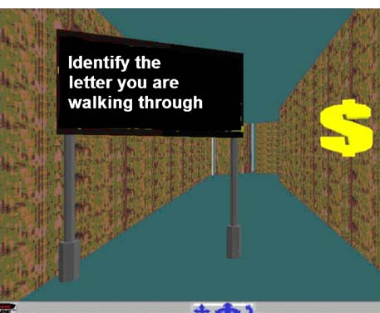
\includegraphics[width=90mm]{images/litreview/dsim1.png}
\caption{Image of dyslexia simulation}
\label{autisim1}
\end{figure}

\begin{figure}[H]
\centering
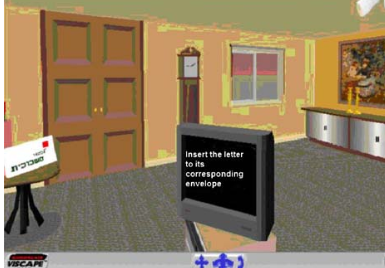
\includegraphics[width=90mm]{images/litreview/dsim2.png}
\caption{Image of dyslexia simulation}
\label{autisim1}
\end{figure}

Results of the study revealed a significant improvement of understanding and awareness in the experimental group whom played the VR simulation.

\begin{figure}[H]
\centering
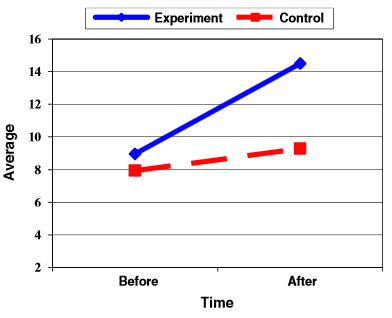
\includegraphics[width=90mm]{images/litreview/dsimresults.png}
\caption{Results of dyslexia simulation}
\label{autisim1}
\end{figure}

Physical disability simulations have been thought to hold disadvantages, potentially lead to pity and misconceptions \cite{dd}, for example the user might take a simulation literally that the experience is exactly what it is like to be all people with, dyslexia for example, rather than a potential representation and experience and understanding that every person is different and will be affected by symptoms in a different way.

A computer simulation may hold an advantage over physical simulations by being possible to depict developed cognitive advantages aspects such as heightened hearing (in the case of visually impaired). In addition computer simulations could highlight thinking differences by visualising the in-game character's thoughts and feelings when approached by various obstacles and these could be used to reduce pity or misconceptions.

In regards to the overall success of simulations, little research has be found to conclude the success or failure of using simulations as a method to raise awareness and understanding apart from \cite{dyslexicsimpar} which also specified "no studies have been made to date, of efforts to increase awareness of the cognitive aspects of the child with learning disability".

\subsection{Autism simulation and tools}

In February 2013 a playable 3D virtual environment depicting sensory difficulties in autism was released. The simulation involved the user navigating a school playground which contained other children whom all looked identical(to represent difficulties with facial recognition). If the user gets too close to the children, visual distortions and high-pitched sounds/screams are played. 

\begin{figure}[H]
\centering
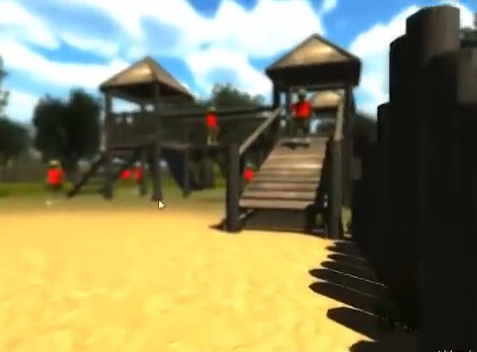
\includegraphics[width=90mm]{images/litreview/autisim1.png}
\caption{Image of playground with no sensory effects}
\label{autisim1}
\end{figure}

\begin{figure}[H]
\centering
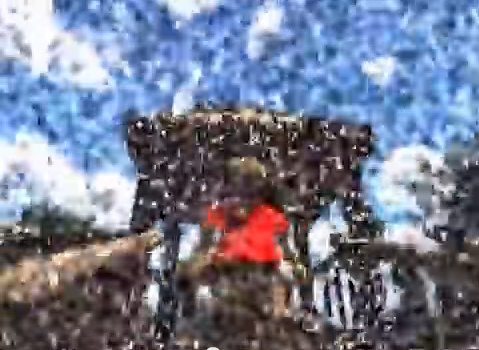
\includegraphics[width=90mm]{images/litreview/autisim2.png}
\caption{Image of playground with sensory effect distortions}
\label{autisim2}
\end{figure}


The simulation from the public was well received and regarded as a good step in increasing awareness and understanding of autism. From those with autism the feedback was mixed with some commenting the portrayal was not an accurate representation of their difficulties whilst for others it was, highlighting the breath of experiences these individuals have and the challenge of the task at hand.

In addition to a playable simulation some autistic individuals have created short videos to demonstrate the impact of sensory problems on their day to day lives and these have been very well received(Gary G. Porter). 
\begin{enumerate}
\item Video simulation of a sensory overload created by a group aiming to use media to help others understand autism: http://www.interactingwithautism.com/section/understanding/sensory/1
\item Video simulation of sensory overload in a supermarket created by an individual with autism: https://www.youtube.com/watch?v=IcS2VUoe12M
\item Autism simulation of a variety of aspects: http://simdis.jisctechdis.ac.uk/Autism/repres.htm
\item Video of sensory overload whilst an individual is walking along a street: https://www.youtube.com/watch?v=plPNhooUUuc
\end{enumerate}

One great benefit of conveying difficulties visually is that it helps obviates to some extent the ever-present language barrier and helping to overcome difficulty for people with autism.  

\chapter{Participatory Design}
Autism as previously described comes with a vast array of difficulties, some of which may be too complex or time consuming to convey(such as social difficulties). It was consequently important to select the most salient aspects of Autism and the participatory design was conducted to facilitate these choices and the design of the prototype. 

\section{LAER Lab}
An initial consultation was held with Learning and Adaptive Environments Research(LAER) Lab which aims to "bring together academics and students interested in technologies designed or applied with the goal of furthering education". In attendance were several members(I have little idea of who these were or how to describe them...you, Alyssa...) as well as two other students whom were also creating software projects related autism. An overview of the simulator was given in addition to goals and suggestions(see appendix for notes on what was given). Children are exposed to a plethora of different environment on a day to day basis(school, work, parks, etc), however, the most common location for a child is the home and thus by understanding the pitfalls and hazards around the house, knowledge should be transferable to other environments or domains. 

The consensus of the group was to restrict the simulator fist and foremost to conveying sensory differences in autism and to focus on the 3D home environment.

// think I still may have the actual document I took in all scribbled on. Or emails/feedback which may give indication of what happened.

\section{Interviews}
Interviews were conducted with five people and varied from teachers as well as adults with autism. Participants were recruited using the LAER labs participant network as well as a attendees to an Autism group.

\begin{enumerate}
\item Candidate one: teacher of a school for autistic children
\item Candidate two: special needs teacher of a school with varying disabilities.
\item Candidate three: parent of a teenager with Aspergers syndrome and ADD. Described themselves as neurodiverse having severe sensory difficulties but fewer social ones.
\item Candidate four: parent of a child with Aspergers syndrome and is themselves neurodiverse. Candidate describes having high sensory issues and fewer social ones.
\item Candidate five: person with high-functioning autism whom has higher social difficulties and fewer sensory.
\end{enumerate}


\subsection{Methods}
Ethical and consent forms were completed and participants all allowed for their interviews to be voice recorded. Interviews with teachers were conducted in the location of the schools. Interviews with candidates three and four were conducted at my own home and interviews with candidate five was conducted at their home. Candidates were in addition shown mock up images of sensory overloads(see figures \ref{sensorymockup1}, \ref{sensorymockup2}, \ref{sensorymockup3}) and asked for their feedback. 

Some interview questions were scripted however the interview topics varied as directed by the interviewees and dependant on the person's experiences i.e a teacher would be asked different questions to someone with autism. As interviews progressed there were improvements on questions asked. Some interview scripts have been included in the appendix however as they were auditorily recorded and some over an hour, not all information could be transcribed. Questions differed depending on the group: teachers were asked more specific questions in relation to their work and their feeling towards to the simulator concept. Adults with autism were asked more personal questions in relation to their own difficulties. 

\textbf{Summary of interview topics for Candidates 3-5}
\begin{enumerate}
\item Opinions and suggestions on the proposed project.
\item Most prominent difficulties faced on a day to day basis(as a parent or individual with autism).
\item In your opinion what is the difficulty that Neurotypical people find the most difficult to grasp about AS children.
\item Obstacles faced around the home environment
\item What would you regard as a successful day.
\item Explanation of sensory or meltdown experiences or triggers.
\item Problems in communicating difficulties.
\item Experiences in contending with mainstream schools.
\end{enumerate}

\textbf{Summary of interview topics for Candidates 1-2}
\begin{enumerate}
\item As you have years of experience with AS children, would you find it helpful if a simulator highlighting sensory difficulties, meltdowns ambiguous instructions was created?
\item In your opinion which topic should be highlighted as the most important within the simulator? 
\item If you had a trainee, what important information would they need to know and what aspects are the hardest to explain.
\end{enumerate}

Finally, all candidates were shown the following mock-up images of sensory overloads and asked for their feedback. 

\begin{figure}[H]
\centering
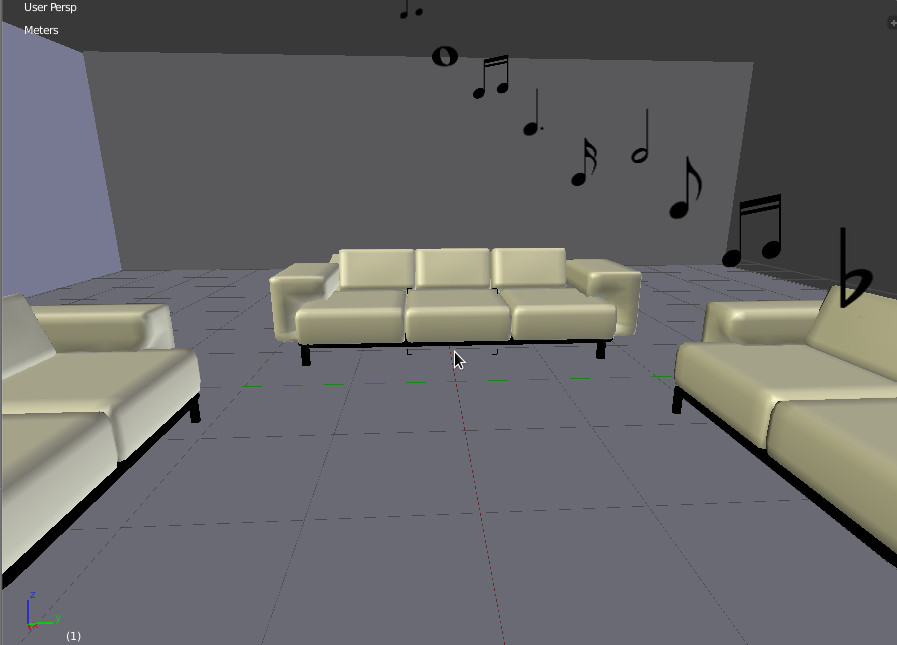
\includegraphics[width=90mm]{images/design/GD_basic.jpg}
\caption{Room with one object generating sound}
\label{sensorymockup1}
\end{figure}

\begin{figure}[H]
\centering
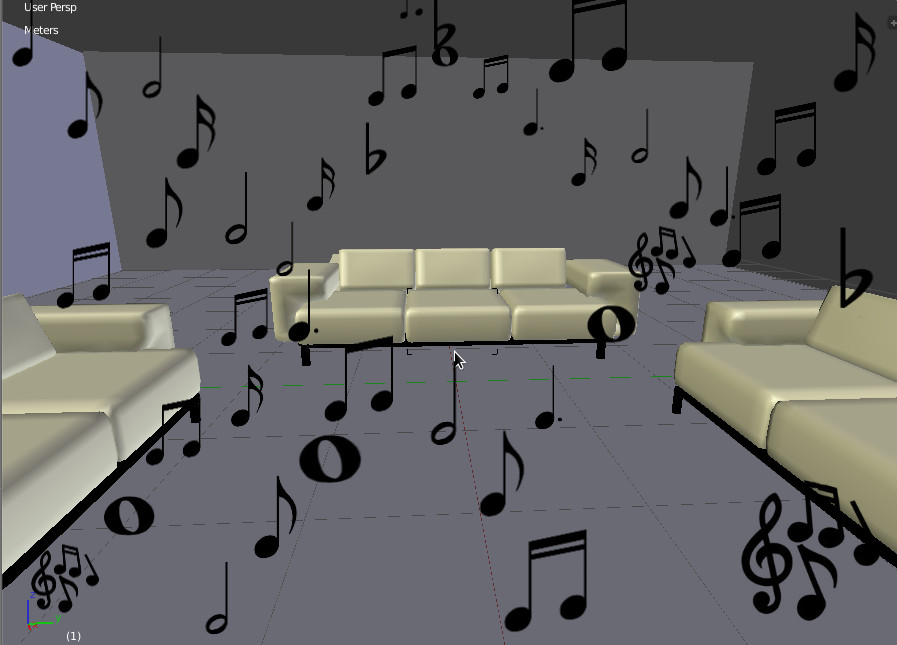
\includegraphics[width=90mm]{images/design/GD_moresound.jpg}
\caption{Effects of multiple objects creating sound}
\label{sensorymockup2}
\end{figure}

\begin{figure}[H]
\centering
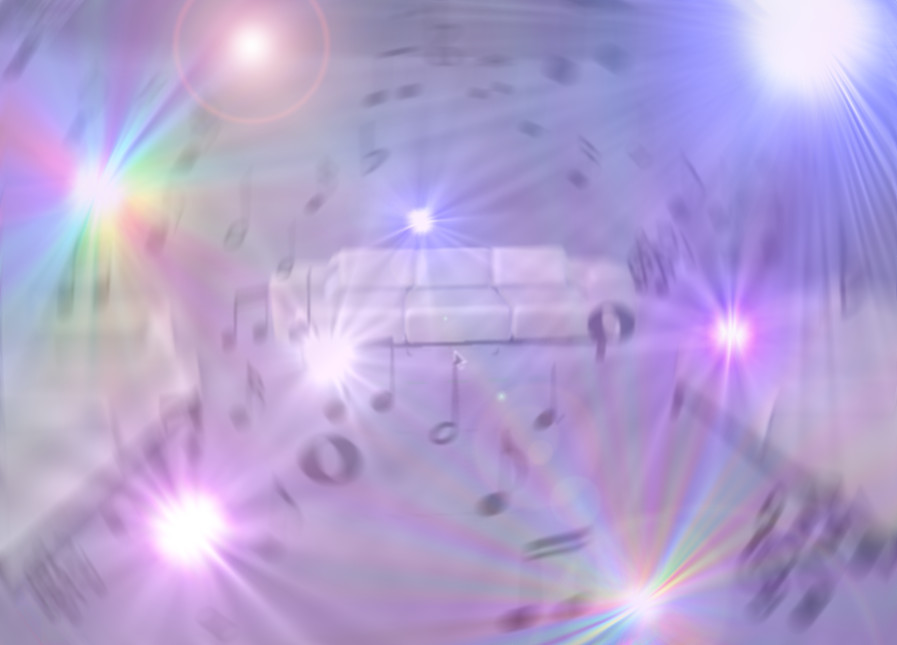
\includegraphics[width=90mm]{images/design/GD_overload.jpg}
\caption{Sensory overload. Lights have become brighter and environment is harder to see. Gaussian filter applied}
\label{sensorymockup3}
\end{figure}

\section{Results}
Interviews were an invaluable contribution to the project that gave insight and feedback into the Autism world currently not found from literature. As interviews were guided by the interviewee, some interesting and finding were observed. In addition, obtaining information from a teacher with large amount of experience in the domain revealed problems when new trainee teachers arrived and how they interacted with children with autism in class.  

Sensory difficulties was particularly prominent for two interviews "I was just so traumatised by the time I got to school with all these different noises, smells in the car and overload of sensory information. I'd just sit in silence and I couldn’t explain to anyone around me what was going on. When I finally arrived home, it just all came out as anger, rage even and my parents never knew why."[C3]. "The noises in the playground were just too much. So i'd sit by the edge of the playground and watch cars go past because those at least were predictable. I used to do this with slinkys on the stairs as well. The sound was beautiful."[C3]. [C4] also specified that for them to replenish energy a quiet environment was required and that "special interests" could be "literally used to replenish energy levels". [C4] in addition specified that as a child they would take coins around with them everywhere they went so they can spin them and use this to alleviate some of the turbulant sensory experiences "I used to do this in school and teachers didn't like that I wasn't paying attention to them. They didn't know that playing with them actually helped me to focus on what they were saying".

[C3] specified they were unable to communicate difficulties until much older however this is contrasted with another interview that felt "I'm pretty good at verbalising my problems, I've always been quite good at doing so although people don't always understand" [C5]. Although the prevalent theme of wanting more understanding was apparent, it was interesting to see the differences in obstacles faced and highlights the need for the simulator to be flexible. 

Changes in routine and structure were also highlighted a predominant cause of stress and anxiety as "A good day would be a structured day with no unpredictable events or changes in routine. Changes in routine can really make me anxious. And when I don't wake up with anxiety, sometimes anxiety can last for days. Also, if the weather is nice, that can help a good day" [C5]

The hardest difficulties highlighted by both teachers was "Language, communication and information processing delay. "A lot of staff have verbal diarrhoea and we have to keep reminding them to give black and white information or time to answer questions. Also the delayed processing of information where staff keep repeatedly asking questions without giving them time to think."[C2] and such events were said to sometimes lead to a meltdown. [C2] also spoke of the difficulty with contrasting sensory needs in the classroom, if a child required visual simulation which manifested as turning the lights on and off it could cause sensory issues for another child whom is sensitive. 


\section{Conclusions: Goals and restrictions identified}
\label{goalsandrestrictions}
2 of the 3 people interviewed specified that found the images of the sensory overloads extremely uncomfortable to view(and quickly looked away), and that it was an accurate representation. This demonstrated that a sensory overload differs for each individual and indicates more should be consulted as 3 is a small sample. However, the projects core aim is to raise awareness of these problems rather than attempting to give an identical experience of having autism and thus the mock images will be used unless feedback in the formative evaluation indicates changes are required. 

From the interviews conducted, the choice of project was solidified as well as the difficulties chosen to convey:

\begin{enumerate}
\item Sensory atypicalities: selected as the primary difficulty to convey due to their prevalence and hidden nature which is less known to the public
\item Meltdowns: As these can be caused by sensory atypicalities and it is important to convey to the user the impact of difficulties, not just the difficulties themselves.
\item Special interests: A means in the game to 'soothe' the character and counteract meltdowns.
\item Information processing delays: commented as a big problem in the classroom.
\end{enumerate}

Due to the complexity of conveying social and communication problems it was decided not to include this in the first version despite its prevalence in autism life. Sensory processing problems were selected as as this was a prominent theme in interviews and listening to individuals speaking of the trauma, the inability to communicate and seek help was really heart-felt. Information processing was selected as teachers highlighted this as a main cause to meltdowns in the classroom. 

Project goals and aims were identified as:

\begin{enumerate}
\item Develop a simulator that allows users to play as an autistic child and thereby experience some of the difficulties/obstacles faced
\item Focus on sensory difficulties but include some other information about autism.
\item Allow the user the ability to obtain useful information on how possible household items/situations can trigger sensory problems as well as how a child with autism might cope with these.
\item Increase understanding and awareness of autism and the difficulties faced.
\end{enumerate}


\chapter{Prototype: Design}
The role of the user will be to play as a child with autism and experience the world through their eyes, obtaining valuable insight and understanding as to what it may feel like to have these difficulties reducing inference and guess-work from literature(probably better explained what I mean in the sound part of "Redesign").

The primary target audience selected are teachers however, it should be developed such that anyone with little knowledge on autism and computer game experience can play and learn. To further achieve this, accessibility is an important consideration and where possible it should be made freely available on-line, making autism training a fun and interactive possibility for all, regardless of budget.  

Finally, instead of creating an overall architecture for the prototype it was chosen to simply implement features and allow the system to evolve due to current limited experience with JMonkey; the architecture would be likely rapidly change as issues arise, voiding any plans or design. For the second iteration of the design; a more in-depth plan detailing components of the system should be created.

\section{Game play}

The user will move around and explores a realistic home environment and be able to interact with objects such as turning off lights, opening and closing doors. Their well-being will be monitored at all times by a $contentment$ gauge visible on screen. Certain actions will result in this reducing, i.e a sensory overload or getting dressed and other interactions such as engaging with a special interest will increase contentment. If contentment drops to zero the player experiences a meltdown and restarts. 

\subsection{Interface and Controls}

Contentment as in the top right of \ref{design_interface_actions} is represented as a "health bar". When the user aligns the cross hair with an object and presses the action button, an interface will pop up with the actions currently available. On the top left of \ref{design_interface_actions} is the tool tip which will change depending on what object the cross hair is hovered over, indicate if there are any actions available. 

\begin{figure}[H]
\centering
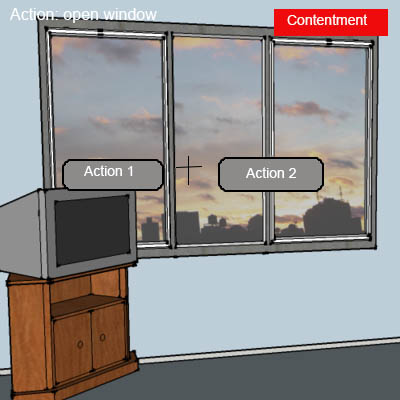
\includegraphics[scale=0.5]{images/design/interface_actions.jpg}
\caption{Mock up of contentment and action selection}
\label{design_interface_actions}
\end{figure}

Controls will be standard game controls commonly found in games. This should minimise learning involved in playing the game,  for current and novice game player alike: 

\begin{enumerate}
\item Mouse or direction buttons will be used to control the camera
\item W: move forward
\item S: move backwards
\item A: move left
\item D: move right
\item Space bar: action button for interacting with objects
\end{enumerate}

\subsection{User tasks: Mission and Explore mode}
Two modes in the simulator will be created, "Explore mode" and "Mission mode". Explore mode offers the user an opportunity to navigate the environment whilst learning how to deal hazards such as sensory overloads and meltdowns with less penalty than in the Mission mode. Explanations, hints and suggestions will be offered as the user has difficulty, for example after the first meltdown an explanation will occur explaining what has happened and that this occurs when contentment reaches zero. On the second meltdown occurrence a hint will be offered as a means to potentially avoid these in the future. In addition, this highlights interview-obtained information that children with high-functioning autism were unable to pinpoint what was causing them to meltdown until they were older and able to verbalise; they had to learn how to avoid situation through experience. 

Mission mode is a game mode that requires the user to complete specific tasks, apply and test their acquired knowledge and understanding from the explore mode whilst circumventing obstacles, in essence, this is the game or story mode of the program. Meta-cognition can be defined as "Knowledge about knowledge" and holds two key elements: Knowledge about knowledge, knowledge regulation which entails formulating plans as to fill knowledge gaps. By implementing the two different game-modes, an environment to learn and then later test it should aid meta-cognitive knowledge development in respect to autism. Users could acquire their own skills and strategies in dealing with these situations, and if some of their conclusions to dealing with these strategies are similar to someone with autism, it will aid understanding as to why some of the autism coping strategies are used.  

For the prototype version of the game, the Mission mode will entail two tasks: To get dressed and then proceed to obtaining a drink from the kitchen and hazards in the kitchen will include lights and a washing machine which will be placed next to the sink. For the first complete version a more in depth storyboard will be created with the aid of feedback from people whom have autism. 

\section{Simulator features}

\subsection{Description boxes}
Users will be able to click on certain objects and obtain information in the form of pop up boxes that may be of interest, hazardous or cause problems for someone with autism. I.e explaining that information on TV may be taken literally and a child may thus expect a toy to react in the same way as advertised or may not be able to identify that what is seen on TV is not real or explaining that clothes can literally feel like sandpaper. This information will be taken from literature and suggestions from people with Autism. 

\subsection{Sensory overloads}
Three sensory-types will be implemented; sound, light and tactile. The proximity and amount of objects around the player will firstly affect the sensory health(which is not visible to the user). When this falls below a specified threshold the first level of a sensory overload occurs and the impact of surrounding objects become more prominent, lights becoming brighter even if they were not initially interfering and causing the sensory overload and the contentment will slowly start to reduce. If the player does not move away, the second level is reached and the contentment bar reduction is rapid; visual effects worsen as the environment becomes more troublesome to navigate; representing a full sensory overload.

Following mock-ups and the positive response, two versions of a sensory overload were implemented and recorded before being sent via email to adults with autism to acquire feedback. The first was not well received or understood, however the second which was much closer to the previous mock images in \ref{sensorymockup3} had a strong positive response.  

One of the effects of sensory overloads was for lights to get brighter which can be easily conveyed in JMonkey using "Bloom" filters. A Guassian filter is suggested to make the overall environment harder to navigate and to mirror dizziness described when experiencing a full sensory overload. 

Finally, the sensory system will effect and be affected by the contentment bar. Interviews showed that if someone with autism is feeling particularly drained from their day or awakens feeling particularly anxious their tolerance to surroundings is lower and hence when contentment is lower, a sensory overload is more likely to occur. If the user is around no interferences or people, contentment will slowly increase. 

\subsection{Meltdowns}
Meltdowns occur when someone with Autism becomes stressed or overwhelmed. This will be represented as 'Contentment' drawing comparison to a "health bar", commonly seen in games. There have been multiple suggestions to convey this:

\begin{itemize}
\item During a meltdown, make the character harder to control. When pushing "right" the character instead moves left and vice versa.
\item Make the screen blackout and reopen with items in the house destroyed.
\end{itemize}

The first option was selected and moulded for the prototype. As contentment gets closer to zero, the camera will shake, giving the player a few seconds to attempt to prevent the meltdown. The closer contentment gets to zero the more the camera will shake. When contentment reaches zero, a meltdown will occur and the player will restart in the bedroom. 

\subsection{Special interests}
'Special interests' were chosen as a way to alleviate some of the difficulties within the environment and replenish contentment. When engaging with a special interest, troublesome sounds will be reduced and if experiencing a sensory overload or meltdown the effects will subsidise. The special interest selected will be a Dinosaur toy which the user can interact with.

\subsection{Information processing delay}
Information processing delay was highlighted in interviews by a teacher as one of the main causes of meltdowns in school. When the user clicks on an object to interact or is expected to give a response, actions will be made harder to select by rotation around the screen. If the character has lower contentment the selections will move even quicker which should result in a greater delay from the player as it becomes more difficult to click them. Such delays could later affect responses from other characters in the game; if the user does not respond quick enough an in-game character such as the parent will prompt the user to hurry up, causing contentment to further drop and the actions to rotate quicker. It was highlighted in the lit review that if someone with autism is interrupted during information processing, they have to start over again but it becomes harder due to stress and anxiety. 

\section{Tool selection}
A game engine was selected to allow focus to be directed onto higher level concepts of the simulator. Suitable game engine candidates as well as modelling tools were identified by looking at those highly rated on gamedev.net (extensive online resource for game developers), whilst taking some previous knowledge into account. After narrowing choices to a few, the advantages and disadvantages were weight up and a choice was finally made. 

\subsection{Game engines}

\begin{table}[H]
    \begin{tabular}{| p{2cm} | p{4cm} | p{6cm} | p{5cm}| }
    \hline
    Engine & Description & Advantages & Disadvantages \\ \hline
    Unity & Unity is one of the most popular game engines available with good support for models. Unfortunately the licence costs 1500 and the free version comes with limitations. & \begin{minipage}{6cm}
    \vskip 4pt
    \begin{enumerate}
   \item Popular game engine to use with a large support base and model repository. 
   \item Quick development with scripting, games with impressive graphics can be made quickly. 
   \item Phone app support.
   \end{enumerate}
   \vskip 4pt
 \end{minipage}   & 
 \begin{minipage}{5cm}
    \vskip 4pt
    \begin{enumerate}
   \item Interface heavy 
   \item Limited to scripting rather than having control of whole game architecture
   \item Costs 
   \item Good computer required to run it efficiently.
   \end{enumerate}
   \vskip 4pt
 \end{minipage}
	\\ \hline
	JMonkey & JMonkey is a java 3d game engine that has been in development around for a few years. It has an extremely active and helpful community, allows complete customisation and holds little limitation being open source.  &
	 \begin{minipage}{6cm}
    \vskip 4pt
    \begin{enumerate}
   \item Provides development environment in addition to a scene graph.
   \item Active community where you often get responses from developers themselves.
   \item Java is quick to develop in enabling focus on higher level features.
   \item Support for online use and phone apps aiding goals of accessibility.  
   \end{enumerate}
   \vskip 4pt
 \end{minipage}  
 & 
 	 \begin{minipage}{5cm}
    \vskip 4pt
    \begin{enumerate}
   \item Java is not seen as the preferred language for graphics or games.
   \end{enumerate}
   \vskip 4pt
 \end{minipage}  \\ \hline
 Panda3D & Originally created by Disney, Panda3D is an engine which can be used via python or C++ although support is mostly for python. & 	 \begin{minipage}{6cm}
    \vskip 4pt
    \begin{enumerate}
   \item Quick to develop for with a choice in language.
   \item Good community with lots of tools.
   \end{enumerate}
   \vskip 4pt
 \end{minipage} &  \begin{minipage}{5cm}
    \vskip 4pt
    \begin{enumerate}
   \item No phone app and limited online support. 
   \item Lack of documentation. 
   \end{enumerate}
   \vskip 4pt
 \end{minipage}
    \\ \hline
    Ogre3D & Ogre3d is primarily a graphics rendering engine and but it does have additional plugins such as 'physics' or drawing interfaces &  \begin{minipage}{6cm}
    \vskip 4pt
    \begin{enumerate}
   \item Lots of modules and plugins
   \item Active support community
   \item Open-source
   \end{enumerate}
   \vskip 4pt
 \end{minipage}
 &  \begin{minipage}{5cm}
    \vskip 4pt
    \begin{enumerate}
   \item Longer development process
   \item Lack of tools such as a scene graph. 
   \item No online support
   \end{enumerate}
   \vskip 4pt
 \end{minipage}
    \end{tabular}
\end{table}

JMonkey was chosen for its active community, development environment being open source and programmed in Java and open-source. Although Java is not seen as the programming language of choice for graphics it enables quicker development than C++ counterparts. Unity allows speedy quick development with great results but the pro version would be required for some features which is very expensive. As JMonkey is in Java put online with ease, increasing accessibility. Finally there were no foreseen limitations with using JMonkey a part from concerns about performance which may become an issue at a later date.

Finally, by selecting JMonkey it is felt goal 4 as highlighted in \ref{goalsandrestrictions} could be further achieved as JMonkey caters for the simulator being put online such that it does not need to be downloaded.

\subsection{Modelling tools}
For modelling there several options available:
\begin{itemize}
\item Maya
\item 3DSMax
\item Blender
\item Sketchup
\end{itemize}

Both Maya and 3DSMax are considered the industries leaders in modelling, animations and effect creation. However, they are both extremely expensive, costing over £3000. Sketchup is a google product, giving a wealth of models however its ease of use for beginners comes at a cost; it is not well supported for games although sketch-up models can be ported to other modelling software and edited to be more suited. Blender is an open source 3D modelling program with quick updates and the choice of tool for many game developers although has been thought to have a steeper learning curve than 3DSMax.

Blender was selected as the primary modelling tool for the creation of game assets, as there is little lost in using it in-spite of being free. It is widely used by game developers and professionals and is the tool JMonkey is most built to accommodate.

\chapter{Prototype: Implementation}
The prototype was created as previously described and was followed by two formative evaluations. One with LAER Lab and the second in the form of an on-line questionnaire after participants watched a video demo. 

\section{Game play}

\subsection*{House environment overview}
The environment consisted of two bedrooms(one empty), a kitchen and a living-room, an overview of which can be seen in \ref{old_house}. It was kept open with no doors and thus no loading required between rooms. The house architecture was designed in sketchup and imported into Blender to be tidied and imported into JMonkey. Some models (such as furniture and the character) were taken from on-line resources such as blendswap.com.  

\begin{figure}[H]
\centering
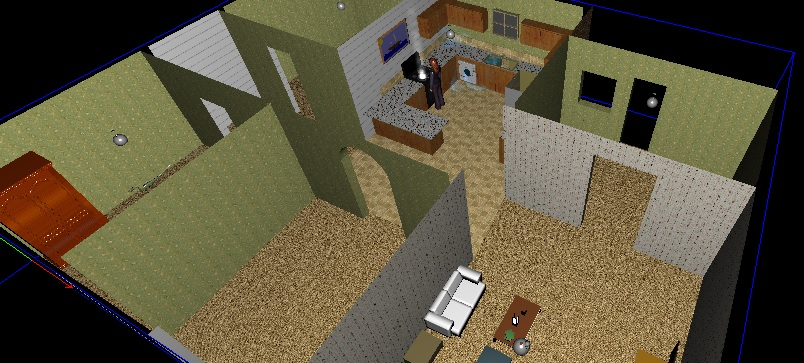
\includegraphics[width=90mm]{images/prototype/old_fullhouse.jpg}
\caption{Overview of the house used in the prototype}
\label{old_house}
\end{figure}

The living room in \ref{prototype_livingroom} contains three interact-able objects, a TV, lamp on the table as well as a ceiling light, the latter two which affect the sensory system and if not turned off or the user is too close can result in an overload. 

\begin{figure}[H]
\centering
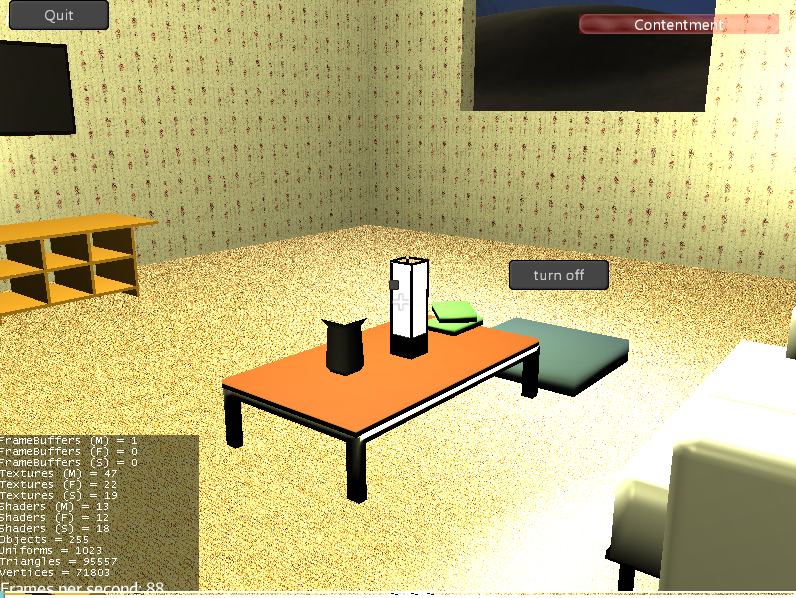
\includegraphics[width=100mm]{images/prototype/livingroom.png}
\caption{Livingroom}
\label{prototype_livingroom}
\end{figure}

The players bedroom consisted of a bed, wardrobe, ceiling light and "special interest"; a dinosaur which the user could interact with.

\begin{figure}[H]
\centering
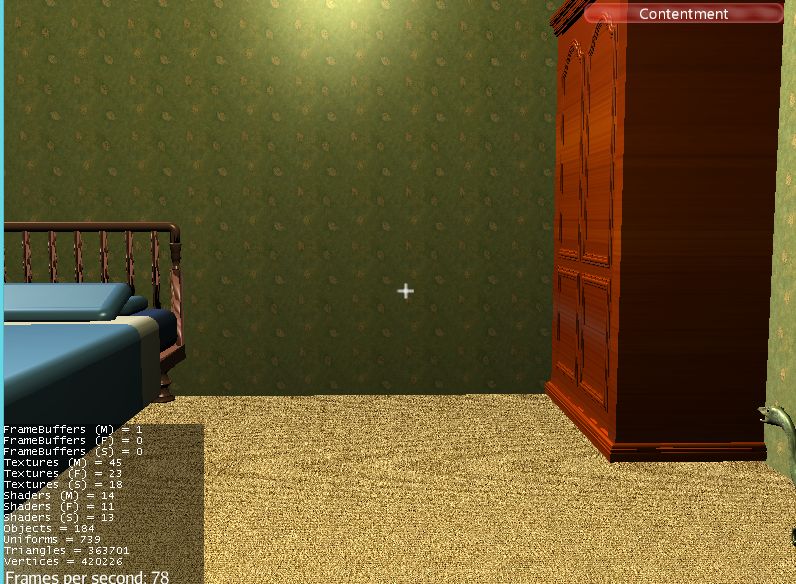
\includegraphics[width=100mm]{images/prototype/bedroom.png}
\caption{Bedroom}
\label{prototype_bedroom}
\end{figure}

The kitchen contained the parent of the game, a washing machine and ceiling light all of which were interactable. The washing machine could be turned on and off which effects the visual effects of sounds. Music notes were primarily to be used in the design, however the wanted effects could not quite be obtained and so sound waves were used instead.  

\begin{figure}[H]
\centering
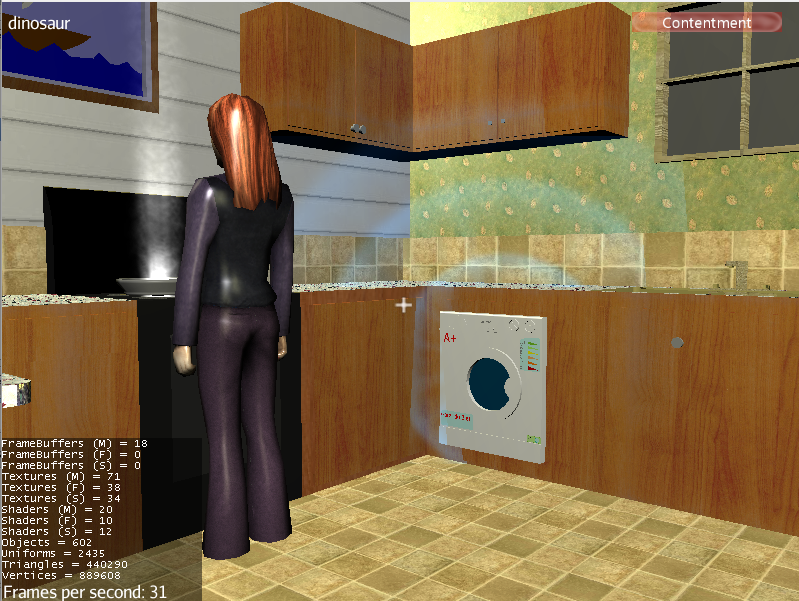
\includegraphics[width=100mm]{images/prototype/kitchen_washingm.png}
\caption{Kitchen: Visual effects from the washing machine can be seen}
\label{prototype_kitchenwash}
\end{figure}

Finally, as the game was open the user could venture outside(useful for running off if a sensory overload was occurring)

\begin{figure}[H]
\centering
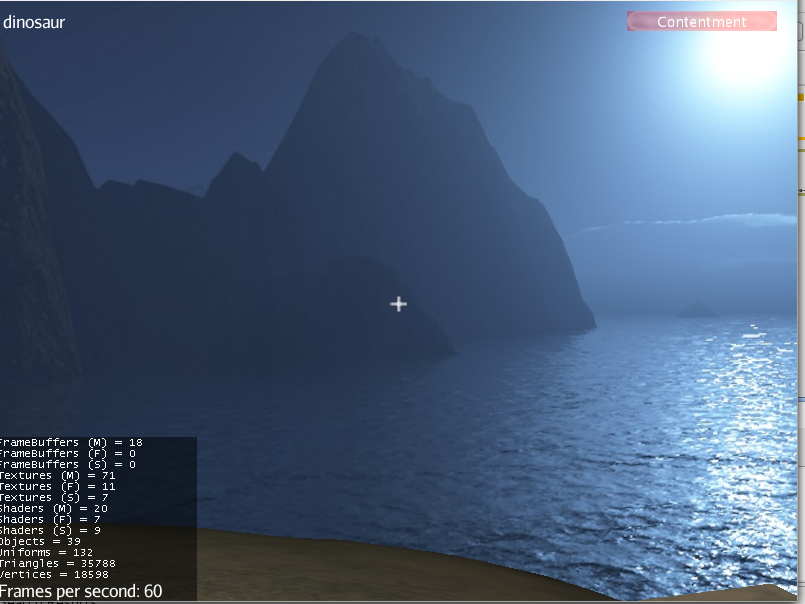
\includegraphics[width=100mm]{images/prototype/outside.png}
\caption{The peaceful outdoors!}
\label{prototype_kitchen1}
\end{figure}

\subsection*{Interactions}

The user can interact with various objects in the scene; some would provide information in the form of description boxes whereas others directly affected game play such as lights and special interests. When available actions appear for selection, the camera is disabled enabling the user to select them with their mouse as can be seen in \ref{prototype_dino}.

\begin{figure}[H]
\centering
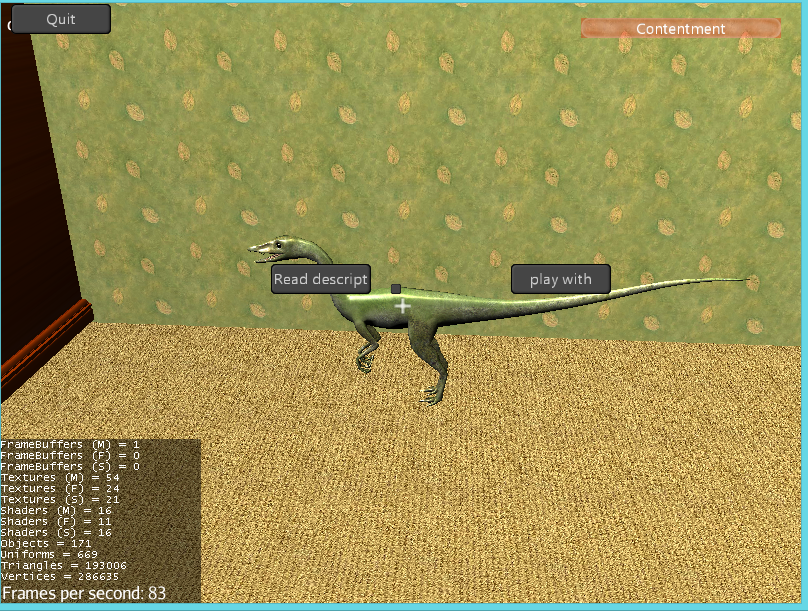
\includegraphics[width=100mm]{images/prototype/si.png}
\caption{Interacting with a special interest. Two actions available for selection can be views}
\label{prototype_dino}
\end{figure}

When the user interacts with the dinosaur(\ref{prototype_dino}), contentment increases although there was little visual indication of doing this(apart from the contentment visually increasing) and if the player was far away from the object, playing would stop. If a sensory overload was occurring and the player moved to the dinosaur quick enough they could prevent a meltdown by increasing contentment although interacting with the object would not specifically stop sensory overloads and should be implemented at a later date. 

\begin{figure}[H]
\centering
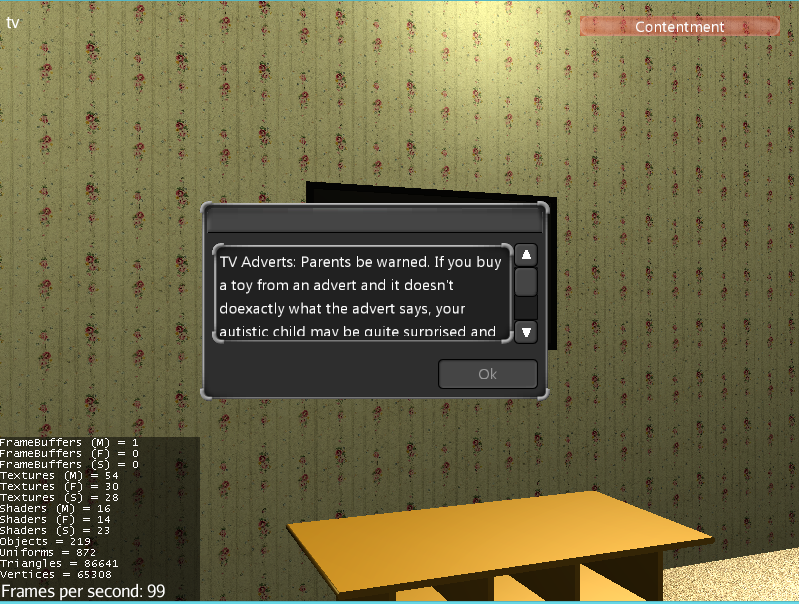
\includegraphics[width=100mm]{images/prototype/tvdescription.png}
\caption{TV description box pop-up, giving warnings of that a child may literally interpret what they see on TV }
\label{prototype_tvdesc}
\end{figure}

Only a few descriptions in the prototype were implemented. Wardrobe, frying pan, TV, dinosaur and one of the issues that arose came during sensory overloads. If one was occurring whilst reading a description the user either had to close it quickly and move away or continue to read and risk a meltdown; which if this occurs the game will reset and the user won't be able to view the description information. This is not ideal behaviour; preventing useful or important information being read.

\subsection*{Sensory overloads and meltdowns}

Sensory overloads occur when being too close to too many hazardous objects and it was was broken down into two stages, the first of which results in lights and the environment becoming brighter as can be seen in \ref{prototype_so1s1} and \ref{prototype_so2s1}. 

\begin{figure}[H]
\centering
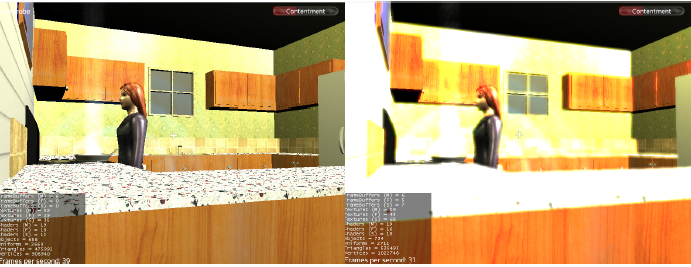
\includegraphics[width=100mm]{images/prototype/old_sensoryeffects.png}
\caption{Sensory overload effects at stage 1: The image on the left demonstrates a view with no effects. The image on the right is the result of the Bloom filter being applied resulting in lights and the environment becoming brighter}
\label{prototype_so1s1}
\end{figure}

\begin{figure}[H]
\centering
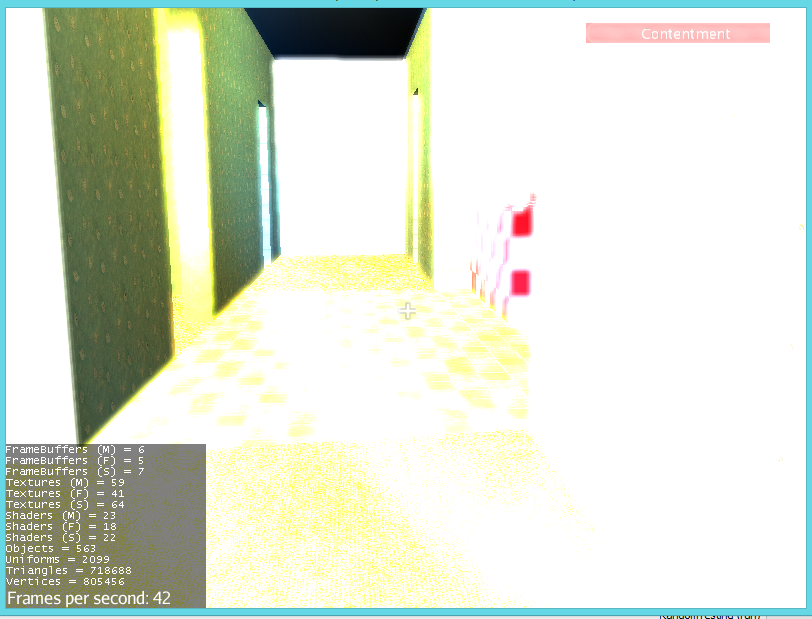
\includegraphics[width=100mm]{images/prototype/hallway_so1.png}
\caption{Sensory overload effects at stage 1: hallway extremely bright as there's lots of lighting causing issues}
\label{prototype_so2s1}
\end{figure}

If the user does not deal with this quickly enough by turning off the source of disturbance or moving away the second stage is entered which can be seen in \ref{prototype_so1s2} and \ref{prototype_so2s2}. 

\begin{figure}[H]
\centering
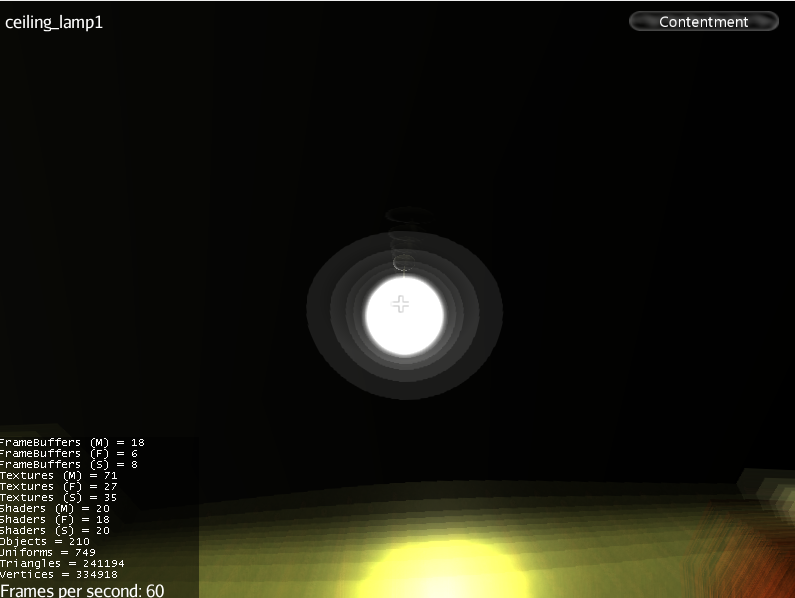
\includegraphics[width=100mm]{images/prototype/bedroom_lightsensory.png}
\caption{Sensory overload effects at stage 2: Light is much brighter and the Gaussian blur filter is applied}
\label{prototype_so1s2}
\end{figure}

\begin{figure}[H]
\centering
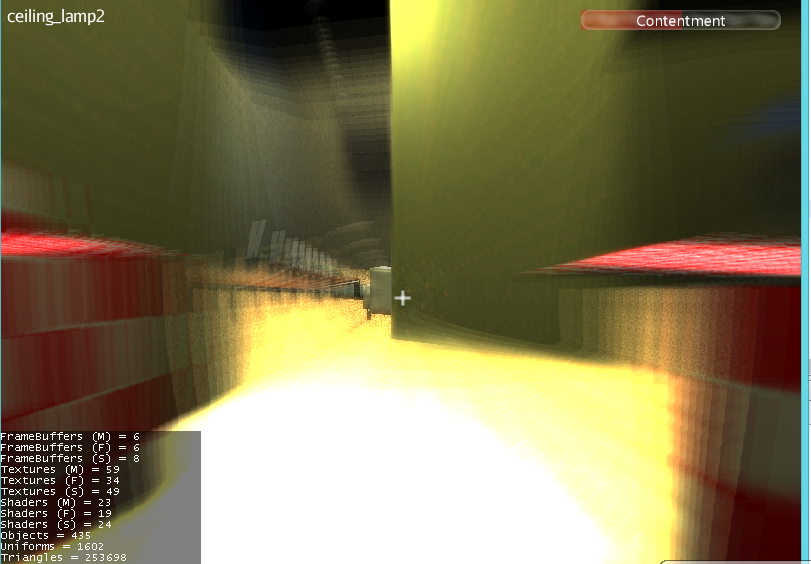
\includegraphics[width=100mm]{images/prototype/so_kitchen.png}
\caption{Sensory overload effects at stage 2: Gaussian blur filter is applied and full sensory overload is occurring}
\label{prototype_so2s2}
\end{figure}

Translating the information from interviews and readings to implementation had proved challenging because of the amount of differing information. The specific triggers do require work and adjustment, for example having only certain types lighting causing problems as currently all of them are. In addition, certain lights should only cause sensory overloads when the user is looking directly into them. Sound is currently represented by visual sound waves emitting from objects and these need to be made bigger and more dense as to cause more visual distortions.

\subsection*{Game modes}
When the simulator first starts the user can select either Explore or Mission mode with a few other options such as "About" and "Help". These cannot be switched during play and the simulator needs to be restarted to change modes. 

In mission mode, two tasks were given: to get a drink and to get dressed. When the user gets dressed, contentment drops due to tactile sensory problems; on completion(assuming the character does not have a meltdown) the next mission is selected. 

Next to the sink as in \ref{prototype_kitchenwash} is the washing machine which combined with the lighting quickly creates a sensory overload. As a representation of "Getting a drink" an action indicator(similar to a health car) is used(see \ref{prototype_actionindicator}) and when displayed the user cannot move. It slowly reduced over time and upon completion the user can move again. Thus, they are fixed at the sink until the action of getting a drink is complete, having a few seconds to run or move away before a meltdown occurs. If the contentment is too low before the task is attempted a meltdown will occur during it and in either case, the player restarts in the bedroom to attempt again. 

\begin{figure}[H]
\centering
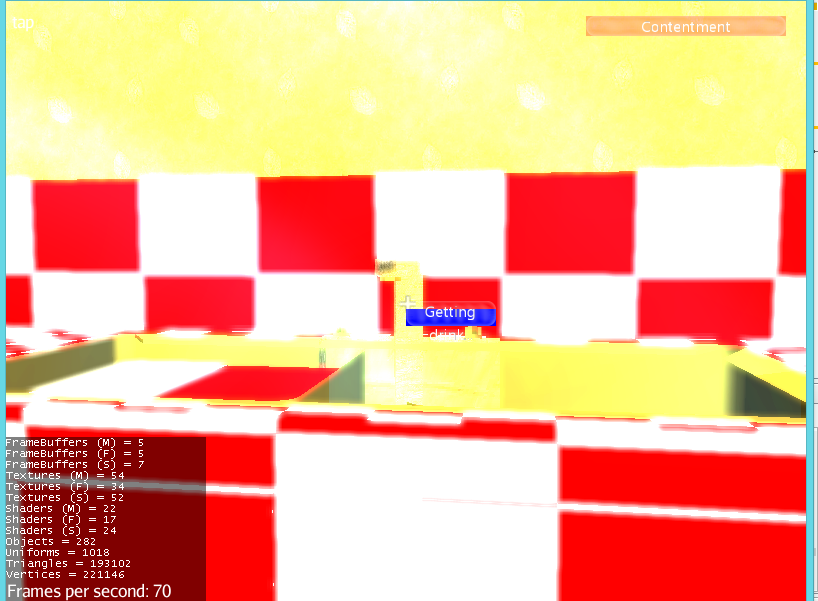
\includegraphics[width=100mm]{images/prototype/actionindicator.png}
\caption{Blue action indicator: (Texture is broken in the prototype when I tried to take this image which is why things are appearing red and white, not hard to fix but no need atm)}
\label{prototype_actionindicator}
\end{figure}

\section{Implementation: technical}

\begin{figure}[H]
\centering
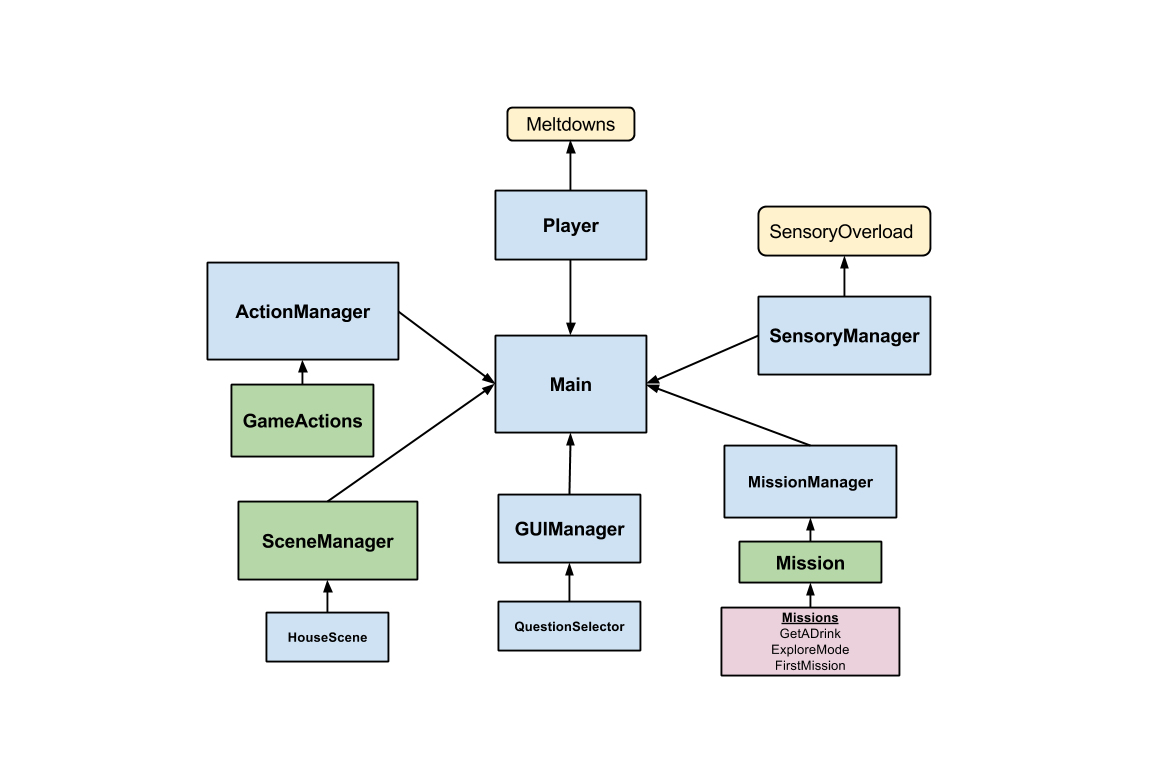
\includegraphics[scale=0.6]{images/prototype/prototypeoverview.png}
\caption{Overview of prototype design}
\label{protooverview}
\end{figure}

The prototype has several main parts:
\begin{enumerate}
\item Main: Contains the main game loop, initialises and updates all other important aspects of the simulator.
\item ActionManager: handles all the actions and interaction the player can do such as turning on and off lights.
\item GUIManager: handles all the GUI. Missions and the rest of the system can make calls to this which decides what and when to display elements. 
\item Player: Represents the player and state of the player in the game(such as current contentment level). Contains methods for internal actions such as "getDressed", calculates reduction in contentment which is dependent on the current state of the player(if not interacting with a special interest or experiencing a sensory overload) and contains methods for starting and stopping meltdowns.
\item SensoryManager
\item SceneManager: Anything that represents a scene extends this and inherits useful methods for setting up a scene. In our case this is a house. 
\end{enumerate}

Terminology used in JMonkey
\begin{enumerate}
\item Spatial: Spatials represent nodes or a geometry in a scene, from a teapot to the root node which contains the entire scene. All models created by blender are converted into spatials. Spatials can be searched and children can be added.
\item Controls: controls are game logic components which are added to control spatials. For example, a movement control could be added to a dog spatial which would repeatedly make it walk around. Multiple controls can be added to spatials making it a very modular feature that JMonkey offers. 
\item AbstractState: can be used to control game logic and are only active once they are attached to JMonkeys state manager.
\end{enumerate}

\subsection{SceneManager}
In JMonkey, scenes are created by adding spatials to a scene file which has the extension of .j3o. All models created in blender area converted to .j3o files and can be translated and rotated in order to create the scene by using JMonkeys inbuilt scene graph. The scenes are loaded into the asset manager which can be accessed by the scene that is loaded which in our case is the HouseScene. A new scene is created by specifying the Scene.j3o spatial name and upon initialisation it would load all the spatials(models) into a hashmap <String, Spatial> so that the rest of the system had quick access to spatials by their key(name of the object) and would thus not have to constantly search the scene graph to find objects of interest which could later be an optimisation issue. 

"SceneManager" is an abstract class so new scenes could be easily created and could use methods that would be commonly required and could setup requirements such as:

\begin{enumerate}
\item Descriptions to objects such as the fryingpan, wardrobe and tv which would appear as description boxes. 
\item The player starting point and respawn point after a meltdown must be set by the scene. 
\item Sensory object types and adding these to the sensory manager for computation when the scene was loaded. 
\item Setup custom materials that may be used in the scene
\end{enumerate}

The SceneManager contained methods such that common sensory objects were created on initialisation based on the name of the spatials rather than needing to constantly use addSensoryObject methods. The SceneManager would go through all the objects in the scene and found ones that had the name "lamp" and would then assign this as a light sensory object and add point lights saving a lot of work for the developer creating new scenes and scenarios. Pointlights had to be added to root node the the scene in order to make sure lights affect all models around it otherwise it would only influence the node it was attached to, for example if attached to a lamp only the lamp would be lit and not the surrounding objects. The better alternative to adding point lights would be to create materials in blender to represent the lighting however this was a lot of modelling work; the problem with pointlights is that it doubles the amount of vertices in the scene for each one added.

\subsection{GUIManager}
At the time the prototype was developed a new GUI package became available for JMonkey. Although it is still in beta with little documentation it provided a faster method of creating the GUI and and required components. 

The main game loop calls the update method in the GUIManager. The GUIManager controls, adds and updates virtually all of the interface and elements such as the contentment indicator, action indicator, displaying of description boxes and action selection, storing any selected actions for Main to request. 

The most important aspect of the GUIManager is the control of the "QuestionSelector", a component made for users to select actions or respond to questions from other in-game characters. The QuestionSelector takes three pieces of information: questions, answers and a boolean to indicate whether or not actions should be rotated and is additionally used to represent information processing delay.


\subsection{ActionManager}
The ActionManager can be broken down into the most important methods:

\begin{enumerate}
\item getActions(Spatial): gets the available actions the user can use on the spatial.
\item doAction(GameActionEvent gae): fires a GameActionEvent which simply contains the name of the action and the spatial to act upon.
\item notifyGameActionListeners: notifies all listeners of an action event
\item getType(Spatial s): gets the type of a spatial which defines which actions can be used on it although custom types can be added. These mostly would depend on the name of the spatial, for example anything that contained the name "lamp" would be assigned the "lamp" type however custom types from missions or scenes could be added so that actions only needed for certain missions such as "get a drink" would only be available during the mission.
\end{enumerate}

If the user clicks on a spatial, using collision detection it is calculated which spatial they have clicked on. It would then use getActions(Spatial s) to acquire which actions the spatial has, based on it's type, and send this to the GUI to display the question selection.

Once the user selects an action the GUI fires doAction which decides what to do about it.

\subsubsection*{Types implemented}
*** put this in a table I think and  cleanup with above, doesnl't need a whole section.

If the spatial is of type "lamp", it would call changeLight(spatial) which is in GameActions and the spatial is searched for an associated point light to change depending on it's current state. 

If the spatial was type "sound", a particle emitter would be added or removed from the spatial depending on it’s current state(if its on or off).

If the object was type "play", the action manager would call player.doAction(name). All internal player actions were in the player class, for example stim, getDressed, meltdown, pickup item, eat etc. There was other types for interacting with objects such as doors, but doors were never used in the prototype.

\subsubsection*{Custom actions and action listeners}
Custom actions can be added from missions or from scenes by implementing the GameActionListener which requires implementation of two methods, notify and getCustomGameActions. Below is an example taken from the "FirstMission"

\begin{lstlisting}
    public ArrayList<GameActionEvent> getCustomGameActions() {
        ArrayList<GameActionEvent> actionEvents = new ArrayList<GameActionEvent>();
        actionEvents.add(new GameActionEvent("Speak to", getSpatial("mum")));
        return actionEvents;
    }
\end{lstlisting}

\begin{lstlisting}
    public boolean notifyAction(GameActionEvent gae) {
        if(gae.getName().contains("Speak to")) {
            isComplete = true;
            return true;
        }
        return false;
    }
\end{lstlisting}

This approach was used to provide modularity so that actions and gameplay in missions was not restricted by the system(a developer could create their own actions and interactions) however still ensuring some level of implementation a developer would not have to implement. I.e lights, sounds, etc.

Once the listener is added to the action manager it will call getCustomActionEventsTypes() which would return all the custom actions added from either scenes or missions and allow the user to select a custom action. doAction would then attempt the action which if it was custom would not be found. At the end of every doAction it notifies all gameaction listeners. Thus missions can listen on to what the user is doing and act accordingly. 


\subsection{Player}
The player class contained the players location and general states such as if objects were being held, if we are interacting with a special interest or in a state of a meltdown.

The main update loop of the player is called from the Main class and it constantly checks the state of the sensory manager which could be NONE, MEDIUM, OVERLOAD. Depending on this state the class will use filters to create the sense of a sensory overload or when the user is nearing one whilst reducing contentment accordingly. If in MED a light filter is applied to make lights get brighter and if in a sense of overload both the light filter and guassian filter are applied. The player update loop can be seen in the appendix.  
 
\subsubsection{Meltdowns}
When contentment dropped below 15 a meltdown would start and progressively get worse which would give the player a few seconds to attempt to prevent it. When a meltdown starts the first person camera starts to shake giving warning; and then gets progressively worse to the point the game is not playable. 

Meltdown events were fired after meltdown had occurred and been stopped. Anything that implemented the meltdown listener would be notified. This was so missions could handle meltdowns if wanted to be done in a different way instead of simply forcing the player to restart at a respawn point. It also meant that missions could give custom messages and prompt users or give hints if meltdowns were occurring too frequently.


\subsection{Sensory Manager}

\begin{enumerate}
\item Sensory health
\item Sensory state: state of senses and objects around that are affecting. Has three states: LOW, MED, OVERLOAD which the Player class uses to determine which sensory effects or filters need to be used.
\item ArrayList: containing all the added sensory objects that may affect us, added by scenes or the scene manager (in the case of items being automatically added by spatial name). 
\item SensoryState: sensory state calculated depending on the value of sensory health. 
\end{enumerate}

Overall sensory state is calculated depending on the value of sensory health. Calculation of sensory health is initially set to a maximum of 100 and is reduced depending on the calculation of sensory points and the reduction occurs during the main game loops. Sensory points calculation is explained in greater detail in \ref{sec:prototypesensoryoverloadalgorithm}.

\begin{lstlisting}
SensorySensoryState getSensoryState() {
	if(sensoryHealth < 40)
		return SensoryState.OVERLOAD
	if(sensoryHealth < 70)
		return SensoryState.MED
	return SensoryState.NONE;
}
\end{lstlisting}

if the state is set to Overload: player class will then apply gaussian and bloom filters
If the state is set to MED: Player class will apply bloom filter which makes lights and the surrounding environment much louder
If state is NONE: filters are removed if in effect


\subsubsection{Sensory overload algorithm}
\label{sec:prototypesensoryoverloadalgorithm}
Objects within a set distance threshold are taken with the threshold set by the sensory manager. The distance measure was arbitrarily set.

\begin{lstlisting}
float getAffectingWeight(Spatial s) {
        Vector3f obj = s.getWorldTranslation();
        float dist = player.getLocation().subtract(obj).length();
        if(dist < distanceAffecting) {
            return (distanceAffecting / dist)
        }       
        return 0
    }
\end{lstlisting}

Weights are then accumulated to give "sensoryPoints". Sensory health is then reduced by the point score and sensory points are additionally adjusted depending on the players current contentment. If contentment is low sensory points will be greater and thus the reduction in sensory health is greater. If the player is stimming or interacting with a special interest sensory points are reduced. If it accumulates to give a negative number, sensory health will increase.

\begin{lstlisting}
float getSensoryPoints() {       
        sensoryPoints = getTotalAffectingWeight();
        
        float health = player.getHealth();
            if(health <= 75 && health > 50) {
                sensoryPoints = 2 * sensoryPoints;
            } else if(health <= 50 && health > 25 ) {
                sensoryPoints = 3 * sensoryPoints;
            } else if(health <= 25) {
                sensoryPoints = 4 * sensoryPoints;
         }
        
        if(player.isPlaying() || player.isStimming()) {
            sensoryPoints -=4;
        }       
        return sensoryPoints;
        
    }
\end{lstlisting}

The thresholds and the design was used to allow a sensory overload to be conveyed accumulative as was conveyed in video in literature review of the simulation of person with autism walking down the street and how they experienced the world. Thus if lights started to get brighter, the user could move away and prevent a full sensory overload. Finally, it means that severity of the sensory overload(and how far sensory health has been reduced) will affect how long it will take the player to recover and have the on screen affects reduced. Discussion and justificaton od sensory design decisions can be seen in \ref{p_imp_discussion}

\subsection{MissionManager}
The mission manager keeps track the current mission played, missions completed and all subsequent missions. Once a mission has been complete it will select the next one in the ArrayList. Weights of how much a sensory object affects the user: calculated using a distance measure. Objects further are assigned less of a weight than object closer. It does not take into account the type of object; for example if a certain noise or sound causes the individual more of a problem than others. Light and sound are all treated in the same way.

\subsubsection*{Missions}
Missions are AbstractAppStates and once loaded by the missions manager has defined game logic that comes into effect but only fur the duration of a specific mission. 

"Missions" extend "Mission" which is an abstract class and contains methods that mission states may frequently need with a goal for development of to be as simplistic as possible with no knowledge of the rest of the system required.

Missions must implement three methods:
\begin{enumerate}
\item isComplete: Mission manager will repeatedly check this and when true the mission will be detached and replaced with the next one. 
\item getMissionDescription: returns description of the mission which is displayed in the description box once loaded by the mission manager. 
\item getMissionName: return the name of the mission and is only used on initialisation. 
\end{enumerate}

In addition missions can define custom actions on objects which may only be applicable when the mission is active, e.g, get a drink, get dressed, ask Mum for help by implementing the GameActionListener. Task classes set the conditions for completion such as player the player must be holding a drink or be dressed and on completion the next task is selected and displayed to the user. One of the benefits of missions and tasks comes with testing; specific tasks can be selected and tested and it thus does not require playing an entire story to get to the parts that are required.

\section{Discussion}
\label{sec:p_imp_discussion}
There are some anticipated problems with the sensory overload algorithm, the main one being that by using discrete thresholds it reduces flexibility. In addition objects in different rooms if within the threshold still affect the sensory system and thus lights in other rooms if close to the walls of these rooms would still affect the player. 
However, the main purpose of the prototype is to acquire and overall bigger picture of accuracy of sensory overloads by being able to present and get feedback on the process rather than specific details. The sensory system thus needs rethinking for the first version to allow greater flexibility, take into account differing sensory object types(light, sound, tactile) and allowing individual sensory objects to set weights on how much these objects affect the user thus, alarms can be set to affect the user more than a tap dripping for example; this level of customisation is required as different people with autism are affected by sensory objects in a different way. Some take enjoyment from certain sounds that others fear. 

At the start of the project significant amounts of time were spent trying to import rather than create models. It was a tedious task because small changes to the models required the whole house scene to be remade in JMonkey or
time had to be spent on editing models better work with JMonkeys import system. It also became evident from using Blender that it has a very steep learning curve and is a tool which can take some considerable time to master.
However, in the last two months of the game development process, these obstacles have been largely overcome. Experience acquired, coupled with updates in February to the JMonkey import system, made it easier and less
time consuming to acquire, create, change and import models. The whole scene was no longer required to be rebuilt allowing time to be better spent. Moreover, the update allowed direct use of google sketchup, a 3D modelling
tool which is easier and quicker to use than Blender (although it produces less quality assets) and offers a wealth of free models in the online repository, most of which are home components such as furniture.

Overall, JMonkey has proven to be a good choice. No additional limitations have been found and development was quick once a solution was found to the model import pipeline. The modularity offered by Java allows
further extensions to be created with ease without needing to change a large portion of the program structure. Finally, being able to combine sketchup and Blender has been a great help and with practice, asset creation should
continue to speed up.

\chapter{Formative evaluation: Prototype}
The current version of the simulator has been evaluated in two settings. The first was the presentation of the simulator to LAERLab. The second was a questionnaire sent to some parents/family members of children with autism and adults with autism.

\section{Expert feedback: LAERLab}
The LAER group consists of students and academics with an interest in the field of accessible and educational technology design and 10 members provided comments and feedback.

A short video demo was presented and narrated showing exploration of the environment followed by one task being completed (obtain a drink from the kitchen). The demo included sensory overload effects, meltdown and information processing delay concepts. (**linux died on my laptop that I had used on the day and I'm pretty sure don't have this video!! Unless I sent it to other people via email. Should I just make another? )

\subsection{Results}

\begin{enumerate}
\item Lab members disliked the pop-up information boxes as they felt it interrupted the simulation. It was suggested information may be better put as a sidebar or bottom bar.
\item Made clear that the simulation information provided in the description boxes are just samples of things known to present problems to children with autism and do not represent all children with autism.
\item Idea put forward to allow the user to select the different issues relating to autism and then to test the consequences of this in the environment. 
\item Demo was a bit too quick, one of the problems being the camera is controlled by the mouse and the video was recorded on a laptop (so camera motion was not smooth). The general controls are quite sensitive.
\item Suggestions for tactile sensory when touching objects(create a slightly red blur around the edges as is common in games).
\end{enumerate}


\section{User feedback}
A video demo was briefly put on-line with verbal narration of what was happening in the simulator. No information on goals or target audience was given as users were asked whom they felt it would be useful for. The questionnaire which was completed by 1 family member of someone with autism, 3 parents of children with autism and 3 adults with autism. It contained both qualitative and quantitative questions. Some users chose not to respond using the questionnaire but gave comments. 

*** Reminder to self. Think I saved a massive amount of feedback on this where people didn't use the questionnaire; get from desktop.

\subsection{Results}

\begin{table}[H]
\caption{Questionnaire results. Participants responded giving an answer between 1 and 5. 5 being the highest rating}
\begin{tabular}{| p{9cm} | c c c c c |}
\hline
\textbf{Question} & 1 & 2 & 3 & 4 & 5 \\
\hline
How likely would you be to play the simulator? & 0 & 0 & 1 & 2 & 4 \\
\hline
How much do you think playing the simulator could help you understand the behaviour of a child with autism better? & 0 & 0 & 0 & 2 & 5 \\
\hline
How much did you like the visual effects? & 0 & 0 & 1 & 3 & 3 \\
\hline
How much did you like the graphics? & 0 & 0 & 2 & 2 & 3 \\ 
\hline
\end{tabular}
\end{table}

The qualitative questions asked were:
\begin{enumerate}
\item What is your experience with autism? (for example if you are a parent, professional, family member or someone with ASD yourself)
\item Who would you think the simulator would be useful for?
\item How accurate do feel the representation of a sensory overload is? Please include any additional comments.
\item Do you have any other scenarios, examples or information(that could go in description boxes for example) that could be offered that you think may be useful for others?
\end{enumerate}

Some of the responses to qualitative questions can be seen below, some participants chose not to give qualitative answers and only responded to quantitative questions:

*** appendix with brief summary and analysis?

What is your experience with autism? (for example if you are a parent, professional, family member or someone with ASD yourself)
\begin{table}[H]
    \begin{tabular}{| p{3cm} | p{12cm} |}
    \hline
     Participant & Comments \\ \hline
     1 & Parent of two ASD children. I also have ASD traits which may be aspergers. \\ \hline
     2 & I have a son now aged 15yrs diagnosed at Peterborough aged 3yrs 9 mnts by child development specialist and her team. Who gave enormous help in getting Tom into nursery and then school and regular assessments. We moved back to Ireland my home place when Tom was 6yrs and have had no help since(mistake). Tom has not been in school for more than 3 weeks since age 12yrs due to sensory issues and has recently started taking prozac for anxiety, which has helped enormously! Your simulator is a brilliant idea which will be a major asset to both parents educators struggling to understand a childs condition. There are so many scenes and scenarios that this can cover and it could be extended to outside the home to school and outside spaces! One example - I remember when Tom was about 5/6, we were at the park and it started raining so we headed home as we rounded the last corner Tom stopped and wanted to go back to start of corner! This was repeated 5 times and he was getting more and more annoyed starting to scream. He was insisting we go back again and it was pouring rain, in the end I said thats it and I ran down the road to the house and peered out and he eventually tottered down the road! But it took me ages to figure out what the problem was until I realized it was that every time we started to go round the corner a car came and the engine noise affected/disturbed his action/experience/sensation of something we take for granted and would not notice. A video simulation depicting such sensory agitators would make an enormous difference to carers and how they react to situations. Hope you found my reply helpful I have many examples such as how buttons on his school clothes caused meltdowns every-morning or how the simple task of changing a nappy was hell until we learned to talk the child through in stages. Best regards  \\ \hline
     3 &  I'm autistic  \\ \hline
    \end{tabular}
\end{table}

Who would you think the simulator would be useful for?
\begin{table}[H]
    \begin{tabular}{| p{3cm} | p{12cm} |}
    \hline
     Participant & Comments \\ \hline
     1 & Teachers, teaching assistants, health care professionals, families. \\ \hline
     2 & - \\ \hline
     3 & People who don't know much about autism - eg a teacher with an autistic student \\ \hline
    \end{tabular}
\end{table}

How accurate do you feel the representation of a sensory overloads are? Please include any additional comments.
\begin{table}[H]
    \begin{tabular}{| p{3cm} | p{12cm} |}
    \hline
     Participant & Comments \\ \hline
     1 & I have sensory difficulties so I felt uncomfortable when it became brighter plus the talking. That is me though and I have these sorts of experiences a lot. Not sure how it would feel for someone without sensory issues. \\ \hline
     2 & I think the reactions in the kitchen is good, maybe for other subtle agitators thought clouds could be used! Plus I think the simulator could be used in schools etc in educating young people, but I might prefer to maybe watch as a video if it were possible to have both formats!! \\ \hline
     3 & A lot more severe than how I experience it, but then I've got milder issues than many I know. But the only kids I know who'd go into a full meltdown that quickly from being near a washing machine would be low functioning (eg minimally verbal) so you may want to back it off a bit. (A fire alarm, on the other hand, would get that strong a reaction even from me.) I really like the effect of the swirling options. It's really unexpected, how well it captures what trying to speak when overloaded is like. I'd never have thought of that analogy, but it's perfect. \\ \hline
    \end{tabular}
\end{table}

Please let me know if you have any other general feedback on the simulator. E.g improvements, suggestions or what you would change.
\begin{table}[H]
    \begin{tabular}{| p{3cm} | p{12cm} |}
    \hline
     Participant & Comments \\ \hline
     1 & Felt more could be done with illustrating the pain of noise. Wasn't sure if the simulator did this; I was watching it rather than listening:( Hard for me to do both online. \\ \hline
     2 & - \\ \hline
     3 & Would it be possible to allow the user to chose between 1st and 3rd person mode? I find 1st person really hard to navigate in. \\ \hline
    \end{tabular}
\end{table}

Do you have any other scenarios, examples or information (that could go in the description boxes for example) that could be offered, that you think may be useful for others?

\begin{table}[H]
    \begin{tabular}{| p{3cm} | p{12cm} |}
    \hline
     Participant & Comments \\ \hline
     1 & Try to include some of the good parts of autism as well. For example, I really enjoy sparkly things. If you make him like sparkly things too, maybe you could highlight the sparkly things and make them look extra awesome to show that.  \\ \hline
     2 & - \\ \hline
     3 & I think if you could use the thought clouds as the avi walking around he/she can be expressing discomfort ie hearing unwanted noises etc my son used to be terrified of the vacuum cleaner! So many little things too! \\ \hline
    \end{tabular}
\end{table}


\section{Conclusions}

Following constructive feedback from these sources, the following amendments to the simulator have been selected:

Description boxes: the HUD can to be changed such that information on the environment does not affect game play. Descriptions could be implemented instead as 'thoughts' which would be displayed at the bottom of the screen and when looking at certain objects. An alternative would be to have a 'Task' which would simply enable no other game play apart from exploring and obtaining information on surroundings, whilst still retaining the pop-up boxes. Images could also be included to give better impact for example when explaining that clothe labels can feel like barbed wire to someone with autism an image of barbed wire and the information can be shown.

Meltdown system: contentment needs to simply reduce less when there are sensory problems around the environment although certain sound objects or lights may need to give more impact than others. I.e a fire alarm causing more problems than the sound of the tv. An internal action such as 'close eyes' might also be used. 

Game play: remove mouse for controlling the camera and allow simple arrow direction keys to be used. Also adjust the player movement so it closer resembles walking. Additionally implement an internal action 'run' to allow for faster movement although one suggestion would be for this to increase the chance of bumping into objects of falling over. 

Interface: User instructions for the start of the game need to be implemented as well as menu's and options for enabling or disabling certain sensory effects as viewers with autism commented they found it difficult to watch as it was causing them to have a sensory overload. 

\chapter{First version}
The main focus of the new implementation was to 

\begin{enumerate}
\item Improve performance
\item Improve the game play experience
\item Further modularisation and design for reusable code whilst improving easy of development. 
\end{enumerate}

Large parts of the system were rewritten and improved upon such as the GUI, sensory manager, scene manager. The benefits resulted in simplification of use at the higher level (such as implementing storyboards) and a better representation of the causes of sensory overloads.

Performance issues which were not previously too severe now required direct attention. The game requires a frame rate of 30fps(frame per second) or above in order to be fluent and played without lag. Scenes are required to have a maximum of 100k vertices(from models) with an average of 10-50k. Each pointlight(which is a light the user can turn on/off) used requires the scene to be rendered again and so the number of vertices double with each point light used. Thus, even when keeping within the limits, the amount of lights being used in the game was pushing it to well over a million and the frame frequently dropped below the desired threshold. This was occurring on a computer with a decent processor and graphics card, thus playing on a low-powered machine would not be a good experience.  

Previously a large amount of models from other websites such as blendswap.com with using programs such as sketchup were used to further quicker development but these were found to be exceptionally inefficient at runtime due to the number of vertices. Efforts were spent on improving skills in Blender and what was required to make lightweight game models and as the whole house needed to be recreated, from previous experience too much time was spent on attempting to find models and thus it was decided to do virtually all of this personally so if any further problems arose I would be better equipped to deal with them. Where previously the entire house was modelled and imported, the solution to the above problem was to split the house into individual rooms/scenes with doors that would load unload the current scene and load the next one. Problems to performance caused by point lights is reduced as a single room only needs to be rendered again and not the entire house and this approach further allows for more detailed models as it would not affect the entire scene but a single room.  

The result of the restructure meant the FPS improved tenfold, from an average of 30fps to 200-400fps. If any objects were found to be creating problems from being too detailed or not textures properly, they could be removed without impacting on the rest of the scene.

Finally, additional benefits from compartmentalising the house into rooms arose for dealing with the model pipeline; it was far easier to load a single room into JMonkey than to load an entire house and fix any issues with materials, textures or general JMonkey importing problems.

The result of the restructure resulted in a drastic improved FPS, from an average of 30-60fps to 200-400fps. If any objects were found to be creating problems from being too detailed or not textures properly, they could be removed without impacting on the rest of the scene.

\section{Planning}

Following the prototype which had little story or goals, a more in-depth story and set of tasks were created, the house was planned and sounds were recorded.

\subsection{Storyboards}
The user will play as an example "Day in the life of a child with autism". This will be split up into several "Missions". The initial story was developed with consultation from an individual whom gave initial interviews. 

\subsubsection*{Mission 1: Complete morning routine}
Complete your morning routine in the designated time(the more out of time, the more contentment drops). Player starts in the bedroom which is a designated safe place/sensory room. 

Routine to complete: eat breakfast, brush teeth, get dressed.

\textbf{Game points}
\begin{enumerate}
\item User progresses to the kitchen for breakfast. Possibly use a particle emitter to make lots of ‘germs’ appear in the kitchen.
\item After breakfast the user must go to the bathroom and brush teeth which reduces contentment due to bristles harsh texture. Noise from the toilet scares and prompts the the user to run out of bathroom into the hallway.
\item The lamp in the hallway however has now been turned on and the hallway looks different, the light causes discomfort. The character freezes and the player is unable to move forward but can move backwards. The user can turn the lamp off at the plug but at this point may not be aware of this. If a meltdown occurs, start back in the bedroom with a message that you can turn the lamp off at the plug. When the user returns from a meltdown contentment will not be at its maximum.
\item User clicks wardrobe to get dressed, information displays explaining that certain clothing can feel extremely uncomfortable for someone with autism and can be compared to sandpaper.
\item Morning ends in the bedroom with player not wanting to leave (the plug to the lamp is away from the bedroom so the player has to pass lamp to turn it off) and trying to play/recuperate. Parent then comes in and says “Cmon, we need to go out!”.
\item Child has a meltdown, thoughts flood the screen with fears and anxieties. Where are we going? Are we taking the car? When will I be back? Stomach hurts, stomach hurts - words become even more jumbled. They weren't warned and thought they could replenish energy levels in their room, the change means the rest of the day could be faced with countless unprepared fears.
\end{enumerate}

\subsubsection*{Mission 2: Afternoon, find out the cause of stomach pain}
Mission is to find out why the characters stomach may be hurting which also gives the user a chance to explore. Contentment slowly drops until the solution is found. Reasons for the pain could be:

\begin{itemize}
\item Hunger/Thirsty
\item Upset stomach or cramps
\item Toilet?
\end{itemize}

The user will be expected to attempt all of the above(the final one the user finds will always be the cause). During the above the door bell will unexpectedly ring and a new character will enter, the parent's friend. The friend was meant to be meeting you both out but due to the earlier meltdown has come to the house instead. Mum tried to explain in advance but words weren't making sense. The person looks like a stranger and can't be recognised and contentment reduces(touch sensitivity occurring from this stranger?). 

\subsubsection*{Mission 3: Evening, get to bed}
Mission pops up that it is time to go to bed but mum stops you and says you can continue playing. Parent then approaches after an unknown amount of time and informs you to go to bed. Meltdown occurs as it's not the exact time and the characters bedtime routine has been broken.

\subsection{House design}
Following a need to compartmentalise the previous house environment as a solution to performance issues, a new and more structured plan of the house was created. The game description column of the table is information the user will see when they interact with the object and will be displayed as "thoughts":

\begin{table}[H]
    \begin{tabular}{| p{2cm} | p{2cm} | p{3cm} | p{3cm} | p{4cm} |}
    \hline
    Room & Object & Action & Game description & Effects                                                                  \\
    \hline
    \hline
     Bedroom & Dinosaur & Play: Increases contentment by playing with it & People with autism have special interests. These special interests help with xyz &                   \\
    \hline
    & Touchside lamp & On/off: slowly adjust the light so it does not turn off rapidly. Contentment goes up when light turned off slowly & & If the light goes off too quickly, contentment increases slightly but then rapidly declines. Room looks strange/scary as eyes not yet adjusted    \\
    \hline
    & Collections of items & & Explains that children with autism have an obsession/need to complete collections &  \\
    \hline
    & Wardrobe & Get dressed & Explanation that clothes can be compared to feeling sandpaper & Contentment reduces  \\
    \hline
   & Spinny object & & & All noise blurs out. Contentment increases \\
    \hline 
    Upstairs hallway & Fluorescent light & Turn on/off. Same effect as bedside lamp & Explanation about fluorescent lights. Effects are like ten camera flashes in your eyes & Lights flicker and cause a 'high' effect on sensory system. Disorientation if exposed too long. \\
    \hline
    & Mirror & "Look into" & I don't recognise this person. Not normal having yourself peering back at you & Causes dizzy/disorientation because it is an odd image to see. \\
    \hline
    & Wallpaper & & & Make wallpaper material move and cause dizziness/sensory effects. \\
    \hline
        Downstairs hallway & Flowers & & & They can either smell good or bad. \\
    \hline
    & Door bell & Automated: on/off & Nicer sound could prompt the user to play with it. Can cause anxiety as doorbell may mean unwanted people in safe space & If player rings it is fine. If another person, causes problems.
    \\
    \hline
    \end{tabular}
\end{table}

\begin{table}[H]
    \begin{tabular}{| p{2cm} | p{2cm} | p{3cm} | p{3cm} | p{4cm} | }
    \hline
    Room & Object & Action & Game Description & Effects                                                                  \\
    \hline
    \hline
        Kitchen & Washing machine & Turn on/off & Could become transfixed with spinning nature & Noisy, need to move away. \\
    \hline
    & Kitchen sides & & Particle emitters to show germs/smells & Reduces contentment \\
    \hline
    & Frying pan & & & Sounds, smells, contentment reduction \\
    \hline
    Living room & TV & Turn on/off & Description indicating that child may think items on TV are identical to what they will get & TV being too loud may hurt. \\
    \hline
    & Hoover & & Description indicating that the noise from Hoovers can be painful & Sensory problems when turned on \\
    \hline
    Bathroom & Bath & Empty bath & & Horrible/scary noises. \\
    \hline
    & Tooth brush & & & Brushing teeth causes contentment to reduce. \\
    \hline
    \end{tabular}
\end{table}

Light switches were added as prior the user would have to click on the object itself. A distance measure was added to actions to make sure that users were close enough to the objects to interact with them. This was necessary for the morning routine and unexpected light turning on; otherwise users would be able to turn it off at a distance which is unrealistic and makes it easy to avoid.

\subsection{Sounds}
One of the tasks in moving from the prototype to the first version was to create a more immersive environment, the addition sound was felt to promote this.

Research was first conducted to find which sounds may be problematic for someone with autism, this was a difficult process involving guess-work and then requesting feedback. It was challenging to put oneself into the shoes of someone with autism and identify what sounds around the house would cause issues. The solution came by finding adults an autism whom would be willing to record sounds around their house that they personally find troublesome. This gave far more indication than words. Previously for example "I find the bath a problem" was misinterpreted as it was thought the noise of the bath plug when pulled that was causing issues, but for one adult it was actually the running of the bath itself in addition the the plug.

Sounds recorded were:

\begin{enumerate}
\item Hoover - Planned
\item Humming from the fridge - Unplanned(recording not great)
\item Light switch turning on
\item Kitchen light sounds(it is a fluorescent light)
\item Washing machine - Planned
\item Dog barking - Unplanned
\item Toilet flushing - Planned
\item Dog drinking - Unplanned
\item Sounds of walking up stairs - Unplanned. Replaced with general footstep noises
\item Brushing teeth - Planned
\item Doorbell - Planned
\item Drinking - Planned
\item Heating/boiler - Unplanned
\item Filling up glass - Planned
\item TV noise - Planned
\end{enumerate}

By asking someone with autism to record the sounds themselves, it personally gave me an experience of the types of things they hear and thus revealed what I needed to convey rather than using guesswork. Sounds such as the humming from the fridge were never considered until the results of the recordings came. Some of these will not be incorporated into the first version, but left for a later date. 

\section{Implementation}

Small game play elements added; selecting actions to interact with objects is now less intrusive. Prior a menu would pop up and prompt the user to make a selection with their mouse which will now only happen if there are multiple options. No object in the environment was designed to have more than 2 actions at the moment, so when an object has a description it will simply be defined in the mission script to pop up and give information afterwards and only once. 

Descriptions usage was adjusted instead of being removed based on feedback from LAER lab. These are now only utalised in the explore mode when giving user hints after a meltdown has occurred. In replacement of some of the description boxes, thoughts are now displayed at the bottom of the screen when to user is looking at a specific object. 

Overall the project is now nearly 5 thousand lines of code, up from 1200 in the prototype. 

\subsection{GUI Changes}
All components now utilize listeners which was not an inbuilt feature of the gui package and had to be built. However it has allowed missions greater control being able to create their own gui without interfering or causing problems to the rest of the system.

The GUIManager was updated to the GameScreen which is now an app state and so does not need to be called in the main game loop, reducing some unneeded code and it now uses states to keep track of the state of the interface. If a description box is on display, or a question is being asked, the start screen is on or the user is in general game play mode. Screens added such as HelpScreen, AboutScreen and StartScreen. These were build however the information was not added on the Help or About screen and needs to be done at a later date as with the release a video was planned to give information as required. 


\subsection{Sensory System improvements}
Following the feedback on sensory overloads and additional problems discussed, improvements were made to how sensory overloads occurred and were calculated. Previously, objects which could affect the sensory system were put into a Hashable which were then periodically checked for the distance to the player and if in proximity would assign a weight. However, all objects would affect the user by the same weight which was not ideal. In addition, sensory overloads were calculated by discrete values and thresholds, making experimentation difficult. This is changed into a continuous function adding scalability and a flexible means to experiment by simply changing parameters, thus helping to address previous issues of meltdowns occurring too quickly.

\begin{figure}[H]
\centering
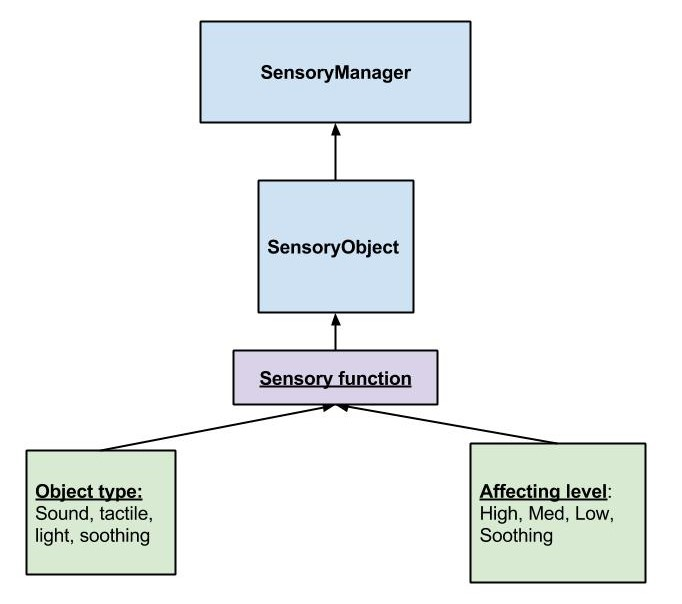
\includegraphics[width=90mm]{images/sensoryobjects.jpg}
\caption{Diagram showing an overview implementation of sensory system}
\label{sensorysystem}
\end{figure}

Each sensory object is given two properties (from the green boxes above) and from this a sensory function is applied and a weight for each object is calculated. The sensory function is an exponential: the higher the affecting level the higher the weight returned and if the object is set as a 'soothing object' a negative value will return instead. 

The sensory manager then takes all the weights of the objects that are in proximity and sums them, taking the log of this. If the log is negative there are no objects and contentment replenishes. The result of the summation is then taken away from the players contentment. 

The first change was to create a new SensoryObject type and in here store all the information required for the sensory objects. 

\begin{figure}[H]
\centering
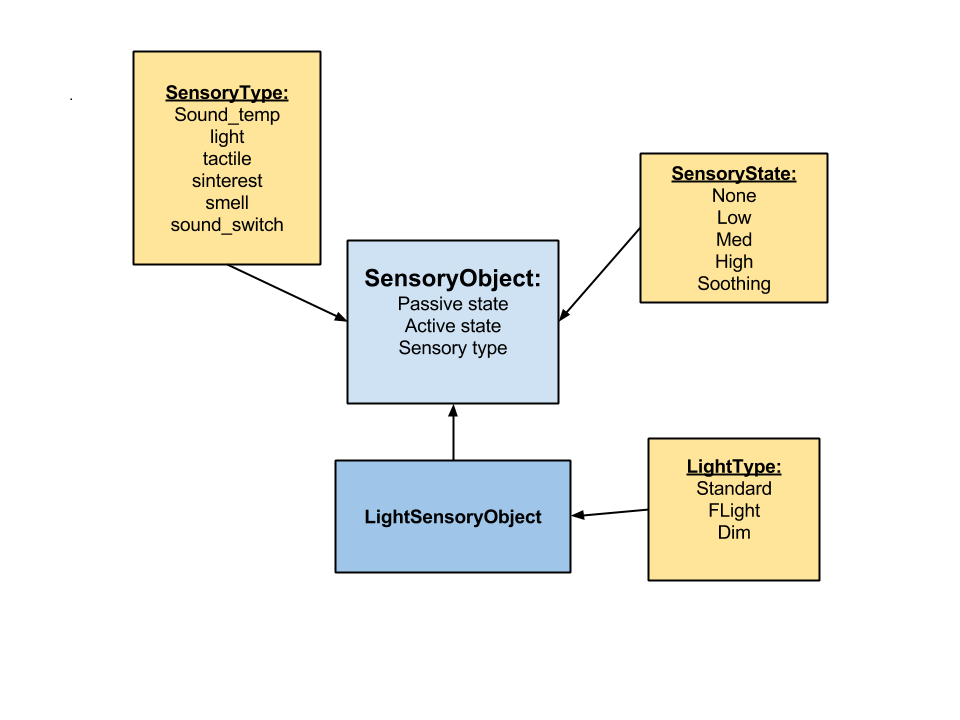
\includegraphics[width=90mm]{images/implementationfirst/sensoryobject.png}
\caption{Diagram showing an overview of sensory objects}
\label{sensorysystem}
\end{figure}

Sensory objects have the following important fields:
\begin{enumerate}
\item SensoryType: The type of sensory object it is. The type will impact what happen when doAction is called.
\item SensoryState: Available states the sensory object can be in. 
\end{enumerate}

LightSensoryObject is an extention of SensoryObject with its own additional set of methods and types. FLight represents a flurescent light and if set the bulb of the light will constantly flicker when it is turned on.

\begin{description}
\item Soundtemp: Object will only temporarily play and then remove itself.
\item Light: Object is a light object
\item Tactile sensory object
\item sinterest: object is a sensory object and will give a negative weight
\item Soundswitch: object is sound and a switch and the user can turn it on or off.
\end{description}

Sounds were the final addition to the sensory manager. When acting on the toilet it now flushes and the alarm clock in the room rings. Sounds create a more immersive environment and an additional layer for creating sensory overloads(i.e making objects more high-pitched). 

In addition each sensory object has two important methods
\begin{enumerate}
\item  doAction which will decide how to act on the object depending on its type when it is called. Each sensory object has three sensory states: current state(the one that is currently set), passive state(effect when the object is off) and active state(effect when the object is on). 
\item getWeight: takes the current state and returns a value weight (also later referred to as the sensory function)
\end{enumerate}

The benefits of representing objects in this way is that the developer can simply create a new SensoryObject from a spatial, set it's properties and how it behaves:

\begin{lstlisting}
        Spatial hoover = livingroom.getSpatial("hoover")
        if(hoover != null) {
           // set the object as a sound switch(it's not constant and the user can turn it on and off.)
            livingroomHooverSO = new SensoryObject(hoover, false, SensoryObject.SensoryType.SOUND_SWITCH, SensoryObject.SensoryState.NONE)
           // set state to high when it is turned on.
            livingroomHooverSO.setUpperLevel(SensoryObject.SensoryState.HIGH)
            // assign the audio that is associated with the object
            AudioNode hooverNoise = new AudioNode(am, "Sounds/vax.ogg", false)
            // add the sound
            livingroomHooverSO.addSound(hooverNoise, (Node) hoover)
            // add the sensory object to the livingroom scene. 
            livingroom.addSensoryObject(livingroomHooverSO)
        } 
        
        Spatial bedroomLamp = bedroom.getSpatial("lamp");
        if(bedroomLamp != null) {     
            bedroom_lampSO = new LightSensoryObject(bedroomLamp, LightType.STANDARD);
            bedroom_lampSO.setUpperLevel(SensoryObject.SensoryState.NONE);
            bedroom.addSensoryObject(bedroom_lampSO);
            bedroom.addLampLight(bedroomLamp);
            
        }    
\end{lstlisting}

Further, the action manager no longer has to find object and calculate what to do about them. It now simply sees that it is a sensory object and calls doAction which will then decide what do about it consequently reducing a substantial amount of code in the action manager allowing the developer to focus on higher level attributes. 

Finally, meltdowns were changed to allow for two different meltdowns, "Freeze" and "Fight". These could be set in missions, fight was the same as previous however "Freeze" would simply make the character freeze and become unresponsive. When a meltdown occurs a radio noise is played. This was partially because of reports of when sensory overloads are bad it can sound like a radio tuning in and out, however it was primarily to create a horrible noise to encourage the user to prevent meltdowns and create an unwelcomed state. The radio noise itself does feel will need to be changed and ideally it would be done with a better sound or audio system; taking all affecting sounds and combining to create a sensory overload effect of tuning in and out. This is left as future improvements however as experience with sound development and creation is lacking and this is thus not time efficient. 

\subsection{Rewrite of scene manger}

\begin{figure}[H]
\centering
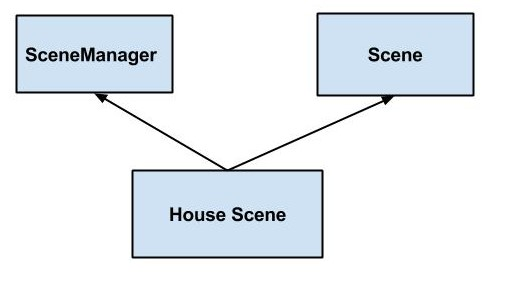
\includegraphics[width=90mm]{images/scenemanager.jpg}
\caption{}
\label{scenemanager}
\end{figure}

The original SceneManager was renamed to Scene. Scene continued to have useful methods for the creation of individual scenes. 

SceneManager now contained tools for the creation, deletion and changing of scenes. The "HomeScene" extends this and contains multiple Scenes which represent the individual rooms. Instead of whole Scene class needing to be created for individual scenes, the class extending SceneManager, "HomeScene" simply needs to specify the jmonkey scene spatial files and set properties of the scene just as points in which the player will appear when it is loaded. 

The HomeScene now implements GameActionListener so it can listen to events occurring in the game and specify custom ones such as needing to load other rooms when users click on doors. The HomeScene can be seen in the appendix.

From the design, some items were not implemented due to complexity or not being necessary at the time. However, some additional objects were created:

Items not implemented:
\begin{enumerate}
\item Flowers
\item Bath was implemented but with no action
\item Collection of items
\item Touchside lamp: although the setup is there and the doAction for when a light object is set to type dim light simply needs implementing(although a fluorescent light was later implemented).
\item Stairs: considered not necessary
\end{enumerate}

Additional items:
\begin{enumerate}
\item Thunder and lightning poster: gives a description explanation unusual fears and autism and that sensory experiences differ for each individual. 
\item Two people in living-room with description of facial recognition problems.
\end{enumerate}


\subsubsection{House implementation}
The additional setup features in addition to the large changes to the sensory manager created an improved way of handling objects. Previously all actions on objects needed to be sent to the action manager to processing but these could now be directly acted upon. 

Below gives some screen shots of the new environment and it's accompanying frame-rates. 


\begin{figure}[H]
\centering
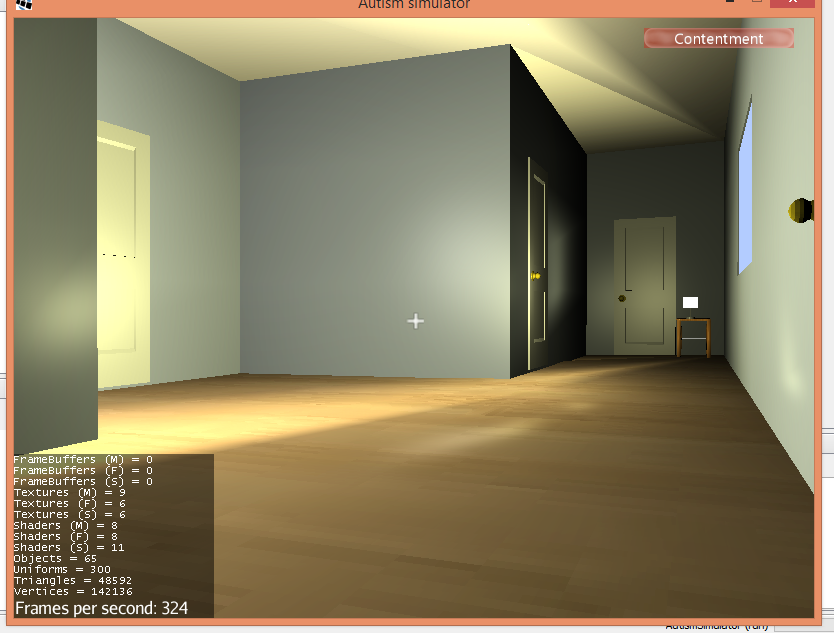
\includegraphics[width=90mm]{images/new_hallway1.png}
\caption{Image of new hallway}
\label{newhallway}
\end{figure}

\begin{figure}[H]
\centering
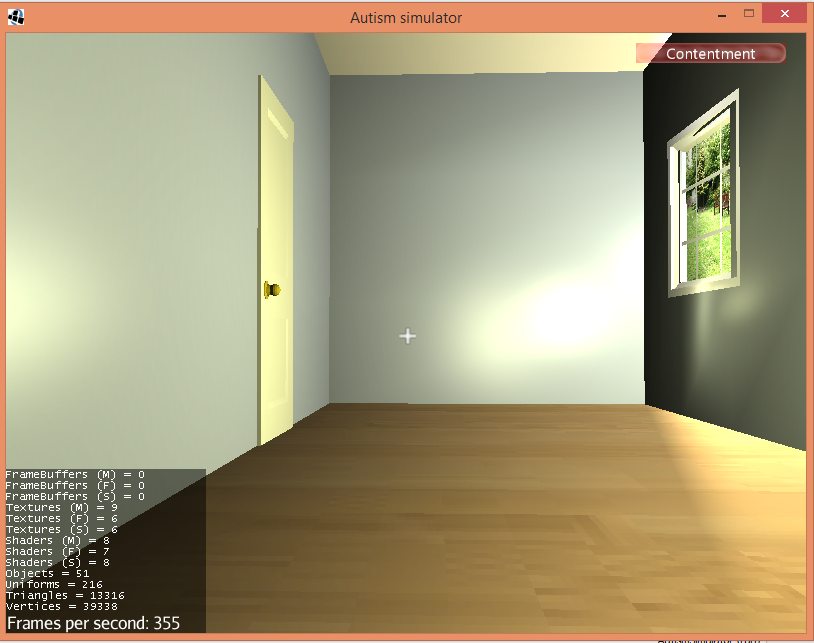
\includegraphics[width=90mm]{images/new_hallway2.png}
\caption{Image of new hallway}
\label{newhallway2}
\end{figure}

\begin{figure}[H]
\centering
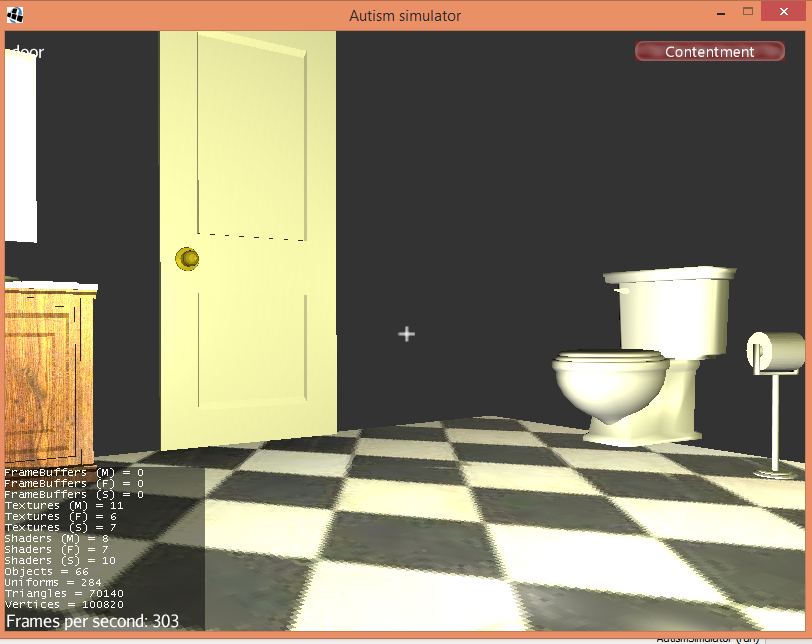
\includegraphics[width=90mm]{images/new_bathroom.png}
\caption{Image of bathroom that was previously missing from the house}
\label{old_house}
\end{figure}

\begin{figure}[H]
\centering
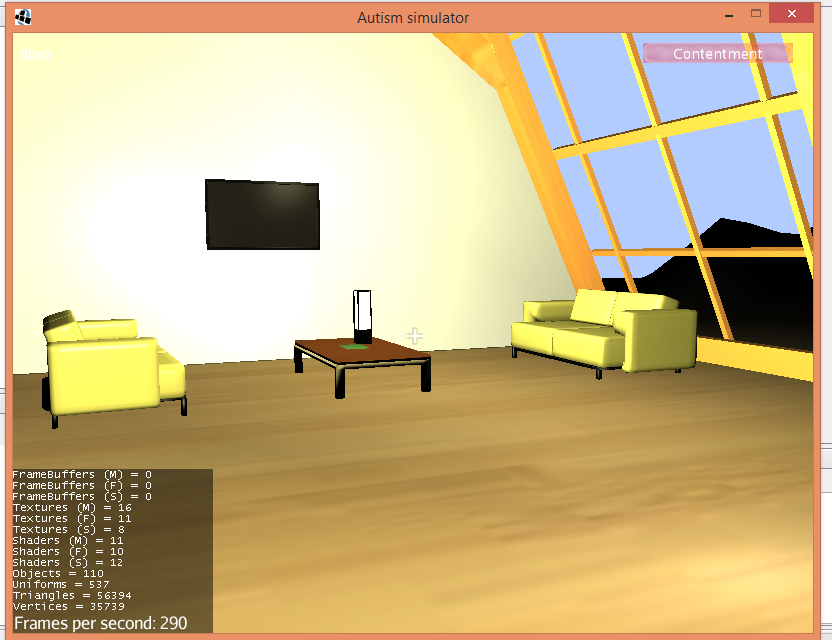
\includegraphics[width=90mm]{images/new_livingroom.png}
\caption{Image of new livingroom}
\label{old_house}
\end{figure}

\subsection{Game state manager}

As the size of the system grew one of the most important changes was the addition of a game state manager enabling universal control and monitoring of the overall system whilst reducing the amount of code in the main game loop. 

The user could now change between "Explore mode"(the user has no tasks and can simply look around the environment) and "Mission mode"(given the tasks or story) without having to restart the simulator although the transition itself was only half implemented with a custom gui. It was not finished due to plans of putting it online where the gui would not be used. However, from this came the addition of the start and help screen and allowance for the user to pause the simulator; common expectations users will have of games.  

The rest of the system can now request useful information from the GSM such as the current mission, which scene the player is currently in and what the state of the GUI is (if actions are being displayed, if the user is required to select an option). If the GUI needs to display information(such as selecting actions) it will notify the game state manager which will halt processes that may interfere. Having a central control made other parts of the simulator easier to develop and reuse since each part of the system only needs to be concerned with the overall game state rather than needing to check a variety of conditions in separate classes.

\chapter{Formative evaluation: First version}
The formative evaluation primarily focused on user experience and game play with a latter goal of making sure the simulation was successful in teaching awareness of at least one attribute of autism. 

Three goals key goals identified for the formative evaluation: 
\begin{enumerate}
\item Check that the game play controls were intuitive with no obvious problems. 
\item Ensure users can complete the first mission without getting bored or too frustrated. 
\item See if user could learn at least one new thing about autism they didn't previously know and ideally what they would learn about or become aware of would be the sensory problems.
\end{enumerate}

Additional goals expected to be obtained through iteration:
\begin{enumerate}
\item Identify areas a user may need help or prompts
\item Obtain qualitative information on how the user was interacting and playing the game rather than their thoughts on the project.
\item Improve users ability to understand the simulator and environment with minimal materials and instructions such future users would be able simply "pick up and play"
\end{enumerate}

Participants were recruited from friends whom although most was aware of the project had not played or previously seen it. The following table gives background information on participants involved in the evaluation and represents the order in which this occurred

\begin{table}[H]
    \begin{tabular}{| p{2cm} | p{9cm} | p{3cm} | p{3cm} |}
    \hline
    Name & Background information & O=Online. P = in person & Location \\
    \hline
    \hline
    Kirstie & Final year chemistry student. Minimal game experience & P & My home\\ \hline
    Robyn & Graduated with a degree in Philosophy and Economics. Minimal gaming experience & P & Own home \\ \hline
    Chris & Final year Masters of Informatics student. Designing an app for visually impaired. Studied HCI & P & Own home \\ \hline
    Ollie & 4th year Social sciences. Medium game experience & P & Own home \\ \hline
    Spyros & Final year Computer science. Studied HCI and was taking Adaptive Learning Environments course and had taken the graphics course. Large game experience & P & My home \\ \hline
    Markus & Final year Computer science and has ADHD. Spent a year abroad working in graphics. Took courses in HCI. Large game experience & P & My home \\ \hline
    Erica & Final year chemistry student & O & -\\ \hline
    Francais & Final year chemistry student & O & - \\ \hline
    \end{tabular}
    \caption{Test}
\end{table}

Participants chosen come from a variety of backgrounds and courses and were felt to be able to give an all round picture of user expectations. With three users being from a computer science background having taken courses in Graphics and HCI they would be more aware of the theoretical pitfalls in interaction and interface design, thinking not only from their own perspective but from multiple users and thus in a good position to offer criticisms and suggestions for solving these problems.

\section{Methods}

Evaluations took approximately 30-45 minutes each depending on the game experience of the user and this time included before and after questions. Qualitative information from participants was extracted owing the small sample statistics. All evaluations took place at either my own home, the participants home. The process was iterative and the system was improved based on feedback depending on the time restraints in between the evaluations.  

Users were asked for their prior experience with computer games in addition to prior knowledge of autism. The first 6 participants were completed in person. The first four participants were verbally asked their their previous knowledge which was written. This was found to be inefficient with some information being lost and thus the later 4 participants completed a before and after questionnaire with the same questions. The final two participants were conducted solely on-line and were sent the questionnaires with instructions and a link to download it. 

Formative pre-questionnaire questions:
\begin{enumerate}
\item What can you tell me about Autism and their difficulties?
\item What is your current skill with computer games?
\end{enumerate}

After questionnaire 
\begin{enumerate}
\item What can you tell me about autism and their difficulties?
\item Did you find the game controls intuitive?
\item Please include any additional feedback or suggestions such as parts you may have found difficult or what you feel could be improved.
\end{enumerate}

No materials were given and users were only told "This is an autism simulator". One of the goals is to ensure the simulator can be played without needing to read instructions and sit through tutorials. This is due to awareness that some individuals will often skip instruction manuals and opt to learn first by experience, later seeking help or consulting guides if they run into difficulty and cannot solve problems out on their own.

Users were directed and encouraged to verbalise their thinking process whilst being observed and given directions such as "Go to the kitchen" or "Go to the bathroom and click on the tooth brush". At a later stage this is expected to change as less directions should be required and will thus be were given on request. If not requested by the user but is was evidence of difficulty the user would be asked "I see you trying to open the door but it is not working. Can you explain how you are trying to do that". Prompts and directions given were recorded on pen-paper for two reasons 1. It could give indication of in-game prompts required for users and 2. difficulties may shed light on alternative ways of doing things or be indication general game-play problems if they arose for other users.

\section{Results}
The system was iterated upon after participant 1, participants 2, 3-4(inclusive), participants 5-6 and again after 7 and 8.

\subsection*{Participant 1}

For the first evaluations the user was just asked to play the "Mission mode" however in-spite of information and instructions at the beginning which were displayed as a description box the participant was finding it extremely difficult and explicit instructions needed to be given. Further problems were quickly identified with entering and leaving rooms; the door model was split into both "handle" and "door" and the user was clicking the handle rather than the door itself which is the norm for most first person games. They were offered to play the explore mode first to become familiar with the environment but still encountered some problems with moving around and quickly experienced meltdowns with some confusion. Once it was indicated that there was a tool-tip explaining actions available when you mouse over objects in the scene, this process became easier. 

For all later formative evaluations users were asked to play the "Explore mode" followed by the "Mission mode" which encompassed just the morning routine as the part that was most tested and ready and could be conducted within the evaluation time-frame. This choice indicated an improvement and users were less confused and were able to all complete the missions. Participants were given additional information that they were to play an "Autism simulator. Use the explore mode and then the mission mode"

Finally key problem identified  was identified; when descriptions and alerts popped up contentment could still reduce so whilst the user would be reading information a meltdown could occur making it further difficult to learn about the environment itself.

Suggested improvements:
\begin{enumerate}
\item Change door model so handle and door are no longer separate spatials. 
\item When hovering over the door with the cross-hair, make the tool-tip change to indicate what the room they will be moving into. 
\item Additional messages explaining causes of meltdowns.
\item Game automatically pauses when description boxes are up
\end{enumerate}

\subsection*{Participant 2} 
Participant 2 was able to comment on some features of autism. Throughout the process they were frequently experiencing sensory overloads and meltdowns and were given prompts on how to avoid these.

Prompts/questions:
\begin{enumerate}
\item To watch the contentment
\item Interact with dinosaur
\item Watch the tool tip to see available actions
\item Needed reminder what the morning routine was
\item Unsure of causes of meltdowns at times
\end{enumerate}

Suggested improvements:
\begin{enumerate}
\item Move contentment bar to middle of screen and make it larger/more obvious. 
\item Put morning routine on the wall for user to look at/observe. 
\item Additional messages on cause of meltdowns or sensory overloads. Messages will change giving a new piece of information each time.
\item Morning routine timer doesn't start until after the description box has been pressed. 
\end{enumerate}

Meltdowns were happening far too quickly to give the user time to think about the cause although it was commented they were really attempting to in an attempt to "prevent that horrible noise". User commented that they felt game play controls were intuitive in-spite of not often playing first-person computer games. 

All suggested improvements were implemented. The rate in which contentment drops was reduced by 20%.

\subsection*{Participant 3 and 4}
P4 went through the simulator extremely quickly and is still to date the only known participant to completed the morning routine without a single meltdown although still commented that this was occurring too quickly. No prompts were required apart from to look at the mill in the livingroom. 

Prompts/questions/comments(P3):
\begin{enumerate}
\item Asking what was causing sensory overloads in specific situations (livingroom where there is a light extremely high up and not obvious)
\item Wasn't clear could interact with dinosaur
\item Wasn't clear when mission was complete with next "Afternoon" routine starting straight away
\item Where is that radio sound coming from?
\item Pointed out that top right were objectives for morning routine
\end{enumerate}

Suggested improvements:
\begin{enumerate}
\item Fix the problem in relation to light objects not on the screen causing overloads.
\item Big, pretty "Mission complete" after each mission with a delay before the next one starts
\item Reduce how quickly contentment drops
\item Increase size of tool tip as not being aware of bedroom object interaction has arisen a few times and this should be the room users should have the most ease. 
\item Adding a drop shadow to thoughts might make them easier to improve.
\item Change meltdown sound from a radio to tv static. 
\item Add text "Objectives" about images for morning routine. 
\end{enumerate}

The first of these was not implemented until after consultation with someone who had Autism and severe sensory difficulties.

The drop shadow could not be added without some difficulty so was left for a later improvement. Contentment was still seen to be be occurring too quickly and the threshold was reduced by a further 30%. 

Finally, it was chosen to include one additional improvement not commented on: a fluorescent light. As contentment was no longer dropping as quickly, and with the removal of sensory "light" sensory objects not being a problem if they were not on screen more "hazardous" objects needed to be added that would be problematic if they were not on screen in order to maintain difficulty. A fluorescent light was selected as they are a highly prevalent difficulty for people with autism. 

\subsection*{Participant 5 and 6}

Participant 6 whom has ADHD offered a good opportunity to test 3 of "additional goals" as they did not to read any of the description boxes or information. Inspite of this very little questions were asked and most difficulties encountered were quickly solved without a need for prompts. P6 was extremely vocal, indicating their understanding of the simulation throughout.

Prompts/questions/comments(P6):
\begin{enumerate}
\item Prompted to move closer to objects when initially couldn't click (thoughts of "I can't reach that wasn't seen")
\item Why don't I like cheese in the kitchen but I like grapes?
\item Prompt to check the routine on the wall.
\end{enumerate}

Prompts/questions/comments(P7):
\begin{enumerate}
\item Why is the tooth brush causing a problem?
\item Didn't notice the mill in the living room could be interacted with which could increase contentment and lesson sensory problems
\item Thoughts still not clear however the JMonkey app statistics were in view which made it difficult to see thoughts.
\item Why is the light flicking in the kitchen?
\item Difficulty clicking on the toothbrush in the bathroom and had to be prompted that it was possible to click.
\end{enumerate}

Suggested improvements:
\begin{enumerate}
\item Information on the tooth brush causing tactile sensory issues. 
\item Add a thought for the mill in the livingroom to hopefully make this more obvious that it can be interacted with. 
\item Description box in explore mode for when the user first goes into the kitchen explaining about Fluorescent lights. 
\item Adjust so that user does not have to directly click on object with cross hair
\item Sizes of thoughts increased in an attempt to combat this without the use a text shadow. 
\end{enumerate}

Option 4 was not implemented and left for a later improvement as it was uncertain how to do this with ease. 

\subsection*{Participant 7 and 8}
Due to not being conducted in person feedback was based purely on answers to the questionnaire and a few general questions afterwards. 

Comments from questionnaires(both participants):
\begin{enumerate}
\item Hadn't noticed mill in living room although commented "I just wanted to get out of there because of the hoover!"
\item Had issues with controls and trying to click in stead of pressing space bar.
\item Trouble clicking toothbrush
\item Visual effects making it difficult to find stimming objects
\end{enumerate}

As the last option is thought to be desirable this wont be a suggested improvement. 

Suggested improvements:
\begin{enumerate}
\item Increase size of tool tip/make it more obvious.
\item Have thoughts as "Boxes" at the bottom
\end{enumerate}

\subsection*{Results summary}
Results for goals 1-3:

\begin{table}[H]
\begin{tabular}{|p{1cm} | p{2cm} | p{3cm} | p{3cm} | p{2cm} | p{4cm}|}
\hline
Name & Controls & Prior autism knowledge & Later autism knowledge & Complete & Comments \\
\hline
\hline
    K & Y & Social difficulties & Meltdowns & N & Controls intuitive but difficulty interacting with environment \\ \hline
    R & Y & Social difficulties & Sensory overloads caused by light and sounds. Meltdowns result in a loss of control & Y & Found myself thinking about the ways to approach the situations and what I could do to prevent that horrible noise \\ \hline
    C & Y & Social difficulties. Special interests & Sensory difficulties. Routine & Y & Thoughts hard to see, add a drop shadow. \\ \hline
    O & Y & Social difficulties & Sensory overloads. Meltdowns. & Y &  \\ \hline
    S & Y & Makes it hard to feel empathy thus hard to understand others feelings and needs &  & Y & Add ability to interact with small objects such as toothbrush without having to aim cross hair exactly at is.  \\ \hline
    M & Y  & Difficulty with social skills. Special interests in maths and a good memory & Routine. Uncomfortable around people, loud noises, bright lights & Y   & Reminder about routine helpful \\ \hline
    E & N  & Affects ability to focus for long periods of time. Social difficulties. People might act in a way that causes them to feel anxious. & Sensor overloads caused by visual, auditory or tactile. String routine required and must not be deviated from & Y  & Wanted to use direction keys to move instead of 'W' key \\ \hline
    F & Y & Aspergers is a form of autism & Visual disturbances due to sensory overloads. Affects emotional response of a person. & Y & Trouble brushing teeth. Visual effect can scupper changes of finding stimming since it is difficult to see what is going on around you \\
     \hline    
\end{tabular}
\end{table}

Full responses from participants 4-8 are included in the appendix. 

\section{Conclusions}
As as consistent with previous research on public knowledge of Autism no-one was able to comment on the sensory issues related although this is a very small sample. Most commented on social or that they knew of the existence of autism and the isolation felt. Clear indication of improved knowledge in each participant is seen by playing the simulator and thus the first goal was achieved. 

Improvements to the process would have been to have verbally recorded the exchange and unfortunately it is felt that some information was lost and a possible cause of some of these issues appearing again in the summative evaluation. By using the on-line questionnaire, information acquired was much more detailed in relation to the goals and feedback was better documented. Most peoples responses after playing the simulator were related to sensory problems and no-one particularly commented on information in description boxes. From this it can be inferred that direct experience is shown to be a better teacher than conveying knowledge in description boxes even though it was in an virtual and hopefully fun environment. Thus a good later addition would be to add more "experience" scenarios such as contending with weather changes or literal language interpretation.  

Game controls were generally found to be intuitive in-spite of having some novice game players. One participant commented on using direction buttons instead but it was chosen not to change this as many games use the game controls used and 1/8 wasn't enough to warrant a change. If similar problems are found later for other users this will be done. 

In-spite of a change in methodology and asking users to play the explore mode with in-game hints offered, users were still finding the task of completing the morning routine difficult; it was found the environment was too harsh and participants were finding it difficult to get become accustomed to controls, think about what was happening, why and develop strategies to avoid, effectively there was too great a cognitive load to be able to direct attention to simply learning and exploring. Contentment was reducing too quickly and meltdowns were occurring too quickly - sometimes the cause could not be identified. The latter part(confusion of the causes) was improved although consultation was required as interviews had specified overloads occurred sometimes without knowing why and it took experience to learn. It was solve by heightening the effects of lights when the user looked at them rather than just being near them.

** dont quite know how to explain this: However, it is felt a degree of difficulty is required to give an incentive for people to find new strategies for overcoming problems facilitating thinking from the perspective of someone with autism, i.e "Ok, i'm faced with these difficulties, but how do I solve them?". By the need to problem solve and find new strategies it is hoped this could further aid teaching as long as there was the understanding that any strategies derived should not be enforced. 

With each iteration of the system it was observed that the types of questions from users were changing and different problems came to light. Instead of asking questions related to "What do I do here?" users were asking questions such as "What's the problem the person with autism has with cheese?", "Why does the tooth brush hurt?". The transition in the way questions were asked can be deduced that the game-play has been greatly improved although more formative evaluations would need to be conducted to see if this is indeed the case. Owing time constraints minimal further improvements were implemented before the summative evaluation. 

It has become clear that not all details and aspects can be necessarily given to users and there were small details such as the mill that some picked up on and others did not. One suggestion was to improve "Explore mode" with an additional tutorial mode potentially with a list of simple tasks that will be ticked off when complete. This will is left as potentially future work.


\chapter{Summative evaluation}
The goal of this summative evaluation to discover if teachers can acquire a greater understanding or awareness of autism sensory difficulties by playing the simulator and to draw conclusions as to whether this tool could be successfully used as a tool for teachers training. 

Two similar evaluations were conducted in person and online with the differences in methodology and participants explained in the alternative methods sections. The in-person evaluations were conducted before the online; with some improvements made in between to ensure on-line users could play with minimal materials as I would not be there to answer questions on game play or give help. 


\section{Methods}
Two vignettes were created in consultation with an expert in Education, Developmental Disabilities, Autism and Technology and entailed a story of a potential classroom encounter with a child whom has Autism as well as potential responses to these situations. Scores were assigned to each response, zero being given for a bad response, 2 for a good response and 3 for the best response.

Participants would be asked to read the first vignette, tick three options indicating how they best felt they would respond in the situation in addition to completing a consent form and background questionnaire on their prior autism experience, feelings towards managing children with autism and computer game experience. Following this they were asked to play the explore mode followed by the mission mode and after playing the simulator participants were asked to complete a second vignette. 

Scores were assigned to the vignette responses with equal amount of answers and points available in the two different vignettes. The order that participants completed the vignettes were alternated to reduce the possibility that one was more difficult than the other affecting the data. In addition, the responses and value were in the same order. The full background questionnaire, consent form and vignettes used can be seen in the appendix.

\begin{table}[H]
    \begin{tabular}{| p{8cm} | p{8cm} |}
    \hline
    \textbf{Vignette A} & \textbf{Vignette B}                                                                                                                                                                             \\    
    \hline
    \hline
    Johnny is eleven years old and has autism. He is in your mainstream class and today you are working on fractions. It is a lovely sunny day and outside someone is mowing the football pitch.  Johnny normally enjoys maths but today he is fidgety and restless.  When you ask him why he doesn't respond.  Eventually he jumps up and leave the classroom without asking permission. & Emily is nine years old and has autism. She is in your mainstream class and today they are doing group projects on using money. Emily's group are annoyed that she keeps taking the coins they are working with and spinning them, and they come to you to complain.\\ 
    \hline
    \end{tabular}
    \caption{Table of the two vignettes used}
\end{table}

\begin{table}[H]
    \begin{tabular}{ |p{1cm} | p{8cm} | p{8cm} | p{1cm} |}
    \hline
    No & \textbf{Vignette A response} & \textbf{Vignette B response} & \textbf{Score} \\                                                                                                                                                                                    
	\hline
	1 & Ask the children sitting near Johnny to go and bring him back in & Tell the children to work it out between themselves & 0 \\ \hline
 	2 & Set Johnny extra maths homework to make up for the lessons he missed & Send Emily outside for disrupting the class & 0 \\ \hline
 	3 & Close the classroom windows & Explain to Emily that the spinning is making it difficult for her group & 2 \\ \hline
	4 & Find Johnny and ask him what is wrong & Ask Emily why she is spinning the coins & 2 \\ \hline
	5 & Call Johnny’s parents and find out what he ate for breakfast & 	Call Emily’s parents and ask them whether she gets any pocket money & 0 \\ \hline
	6 & Send Johnny to the Headmaster for punishment & Tell Emily to stop spinning the coins and focus on her work & 0 \\ \hline
	7 & Offer Johnny a chance to work on his own & 	Offer Emily a chance to work on her own & 2 \\ \hline
	8 & Make Johnny stay inside over lunch to catch up & Take all the coins away from that group &  0 \\ \hline
	9 & Go outside and ask the gardener to stop mowing the lawn & Give Emily something else she can spin & 3 \\ \hline
	10 & Send Johnny to the guidance counsellor & Send Emily to the guidance counsellor &  0 \\ \hline
	11 & Find Johnny and give him a hug & Tell the other children not to bother Emily because she is special & 0 \\ 
    \hline
    \end{tabular}
    \caption{Table of the responses and associated scores for each response}
\end{table}

\subsection{Person}
Participants were recruited from the university of Edinburgh's school of education. An email was sent and participants were asked to email myself with their preferred time. 8 people responded with 2 being unable to find a suitable time. Evaluations were conducted in *Sue's lab, what's it called :)?* and lasted approximately 45 minutes. It was hoped to find more first year or younger teachers with less knowledge on autism however most came from a background of prior knowledge on autism. Owing positive formative evaluation, trial was just on morning routine as there was thought to be more than enough content to aid teaching of autism and the afternoon mission was not well tested. Persons were allowed to ask questions on game-play if they encountered difficulty and these points were noted although few were asked.

Participants were asked to complete the background questionnaire, first vignette and were given little information on the simulator except "you play as a child with autism and get to experience some of the difficulties through their eyes". After playing the simulator participants were asked to complete the second vignette. Afterwards I would answer any questions they had on autism or the simulator itself and take feedback. 

\subsection{Online}

The background survey and two vignettes were put on-line along with a video tutorial which contained basic information of how to use the system and highlighted that no two people with autism are the same and can be seen on http://autism-simulator.com. The simulator was available for downloaded rather than as a java applet due to problems with obfuscation. 

Some improvements made before putting the simulator online: as the tool-tip which reveals what actions are available was not obvious

\begin{enumerate}
\item The tool-tip which reveals what actions are available was still not obvious. This was moved to below the cross hair and thus directly in the users line of sight.
\item Thoughts were made larger.
\item Some bug fixes. 
\item Starting point in the bedroom was moved to a more central location whereas before it started close to the door and one participant was confused of their surroundings for a few moments.
\item Time for the morning routine now counted down 50\% slower.
\item Changes to the start screen.
\end{enumerate}

Teachers were emailed from a previous school I attended and they in turn attempted to find a few other teachers from their school. Teachers were given a link to the website with the following instructions

\begin{enumerate}
\item \textbf{Before} you play the simulator fill out \underline{this} preliminary questionnaire first
\item \textbf{Before} you play the simulator fill out either Vignette A or Vignette B first. I need to have a general equal amount of people doing A or B first.
\item Watch the video tutorial
\item Play the explore mode on the simulator and when you feel ready, play the "Mission mode" of the simulator. If you come across any bugs, please report in the final questionnaire. If you end up completely stuck shut down and restart the simulator by pressing "Esc" key.
\item \textbf{After} you have played the simulator fill out the other Vignette you did not complete first. If you don't I cannot use your data!
\item Fill out the final questionnaire for additional comments and feedback(this part is optional)
\end{enumerate}

The obvious problem with this approach was that it allowed for vignettes not to be completed equally. Some people filled out one vignette and not the other so some data could not be used however this is expected and could have been better designed by an automated system of emailing people the link to the first vignette and a link to download the simulator and after completion of simulator sending an email from the simulator to them with a link to the second vignette. Although possible it was decided not to do this and vignettes have been completed equally.  

The second identified problem could be that teachers could view both vignettes and decide for themselves which one was easiest and complete this first. This could work in the favour of the evaluation if they chose the vignette they were certain of and get this correct and were able to complete the second vignette they may previously have been uncertain of and get this correct. This means that understanding could be increased but the results would not indicate this. However what should be seen is that teacher understanding is not made worse. 

Inspite of these problems it was the first time that gave opportunity to see if people could use the simulator and complete the evaluation without being able to ask questions on game play or if they were stuck. None of the teachers whom completed the online evaluation emailed to ask what they needed to do or ask for help although some emailed they they had issues running the simulator and this was deduced to be due to exceptionally old computers. Required computer specifications thus need to be identified in future work.  

\section{Results}


Below is a summary of total scores and improvements. Full results of answers can be seen in the appendix. 

\begin{table}[H]
    \begin{tabular}{| p{1cm} | p{2cm} | p{2cm} | p{3cm} | p{3cm} | p{3cm} |}
    \hline
    \textbf{No} & \textbf{Total before} & \textbf{Total after} & \textbf{Improvement} & \textbf{First V} & \textbf{Second B} \\                                                                                                                                                                                    
	\hline
	1 & 6 & 7 & 1 & A & B \\ \hline
	2 & 7 & 7 & 0 & B & A \\ \hline
	3 & 6 & 7 & 1 & A & B \\ \hline
	4 & 7 & 7 & 0 & B & A \\ \hline
	5 & 5 & 5 & 0 & A & B \\ \hline
	6 & 7 & 7 & 0 & B & A \\ \hline
	
	8 & 7 & 7 & 0 & B & A\\ \hline
	9 & 7 & 7 & 0 & A & B \\ \hline
	10 & 6 & 5 & -1 & B & A \\ \hline
	11 & 4 & 7 & 3 & A & B \\ \hline
	12 & 7 & 7 & 0 & A & B \\ \hline
	13 & 4 & 7 & 3 & A & B \\ \hline
    \hline
    \end{tabular}
    \caption{Summary of results. Participants 1-6 were in person. Participants 8-12 were online. Participant 13 was in person but completed questionnaire online}
\end{table}

Most came from a very knowledgeable background in autism and may thus be why improvements are only slight. On-line participants were from a variety of background rather than specific autism background and this shows in initial scores. 

From the data we can see that there were either improvements of understanding or in the case where participants already had maximum scores their score remained the same. Unfortunately with participant 5 they only gave two responses instead of three but they did receive the maximum score for both.

For the one candidate whom showed a reduction in overall score, their initial and latter response can be highlighted below:

\begin{table}[H]
    \begin{tabular}{| p{6cm} | p{6cm} |}
    \hline
    \textbf{Response before} & \textbf{Response after}  \\                                                                                                                                                                                    
	\hline
	\hline
	Explain to Emily that the spinning is making it difficult for her group & Set Johnny extra maths homework to make up for the lessons he missed \\ \hline
	Ask Emily why she is spinning the coins & Close the classroom windows \\ \hline
	Offer Emily a chance to work on her own & Go outside and ask the gardener to stop mowing the lawn \\ 
    \hline
    \end{tabular}
\end{table}

From this we can see that their sensory knowledge appeared to have been improved with both related responses given whilst doing the potentially harder second vignette. Thus it can be concluded that although the participants overall score reduced, their knowledge in sensory difficulties in autism increased. 


\section{General discussion}


The first person whom took part in the summative evaluation had a hearing impairment and arrived with an interpreter. Owing a quite a substantial aspect of the simulator experience was the heightened sounds it was uncertain if the full experience would be successfully conveyed. The participant finished in the bedroom unable to complete the morning routine, commenting "It's less stressful to be in here". Afterwards they asked questions such as, "If someone with autism comes to a meeting would you suggest I offer them a quiet room?”. This would be a recommendation and such questions indicate that of not having the full experience the goal was still achieved. This participant in particular was delighted with the system, expressing the need and potential of it. During the evaluation process many participants were found to ask questions and relate their learning to their own experiences.

Participant 8 whom had the vignettes correct initially and showed no statistical sign of improvement specified "I thought this was a great tool and it took me 4 tries to complete the mission. I learnt new things (about fluorescent lights and lights in general)."

It was interesting to observe the different strategies being used by participants to solve the problems. Only one person realised they could look away from the lights in order to prevent a sensory overload(there was no hint for this given). Some people would try to go back to the living-room or bedroom during the routine in order to refill contentment before continuing. It's uncertain as to whether this should be allowed because it's not directly part of the strict routine, but it does convey why children with autism need to be able to use their special interests to deal with the surroundings. Consultations with people with autism would need to be conducted. It could be that the user has a rough routine in the form of goals i.e "Go to kitchen, Brush teeth, Get dressed but they have to develop their own routine to achieve these goals. So, if they get dressed first and their contentment lowers, they now have to complete the rest of the routine with a fixed lower contentment and may find this make achieving the rest of the goals more difficult.

I feel this would be a better way of teaching people about why children with autism require routines. As in the formatives most people commented more on the sensory overloads aspects rather than the need for routine; although through later improvement and focus on learning, of the latter 4 participants, 3 did pick up on the need for routine so it may have been due to previous problems of the environment being too fast paced. However, of these three it's uncertain if the "why" a routine was needed was conveyed over simply the fact "it's just needed to deal with sensory issues"; effectively it is hard to gauge if the candidates acquired declarative knowledge on the topic rather than procedural knowledge.  

\subsection*{Problems}
For in person evaluations most of the improvements were related to those whom did Vignette A first and the participants with biggest responses/improvements both did VA first. This could indicate that vignette B. There also may have been problems with the scoring of the vignettes. For participant 5 of the on-line survey, their responses were "Find Johnny and ask him what is wrong, Offer Johnny a chance to work on his own, Go outside and ask the gardener to stop mowing the lawn. Thus although they received their highest score "closing the windows" which is related to a sensory response. This was given the same weight as decisions not related to responses to sensory. In a broader picture their response is probably a good one however the evaluations goals were designed to look specifically at sensory problems and possibly should have received a lower initial score. Having one sensory related option in B in comparison to two in A could indicate why vignette might be easier however such problems were not found until all of the data was collected. 

The online version lost data due to some people who completed the first and background questionnaire not completing the second. This is unfortunate because quite a few of these participants gave initial low scoring answers and thus it may have been seen there was a large improvement. It can be also be noted that a few teachers with initial low scoring answers expressed they felt that they had good knowledge of autism and were confident of managing behaviours inspite of having not had training. In contrast, those whom seemed to have large amounts of experience of working with autism were expressing less knowledge and confidence in dealing with behaviours when the opposite could be expected. 

Finally background could be skewed as two participants realised they were inverting their responses and needed to redo them. There may possibly have been others who also did this and did not notice. However general background responses seem to fit with the courses taken and courses taken. This was changed in the on-line version so that participants checked boxes for "Strongly agree", etc, rather than having to assign numerical values to responses however the potential for background data not being correct is not seemed strong enough to affect conclusion of results. 

\section{Conclusions}
Improvement was generally seen in participants. A large portion of the participants came with a lot of prior knowledge of autism. Inspite of one vignette potentially being easier it can be concluded that the simulator has not hurt participants understanding of autism and it may have increased understanding inspite of there being no statical increase as was demonstrated in the case of participant 8 and some feedback after the simulator. For the one participant whom had an overall reduction in score; they showed improvement of sensory understanding and thus the goal was still achieved. 

Overall the results are positive although there are not potentially enough participants to reach a firm conclusion. It was extremely useful to see people using different methods of thinking and strategies and it is felt this could be a good platform for discussion of strategies. Some people were very determined to complete it, some people has a bit of difficulty; but they were still very positive about it. However, difficulty of completing the tasks and missions still needs to be reduced such that it is difficult enough to inspire and motivate the user to think of their approaches and potential strategies, but not so difficult that users become frustrated or bored. 

\begin{quote}
Overall this is a genius idea, really useful and I think it could be really good for those working with ASD children and adults (you could also have a child and adult version - are there differences?)” - participant 8
\end{quote}

\subsection{Suggested future improvements}
Suggested future improvements from the summative evaluations:
\begin{enumerate}
\item Allow clicking of the mouse and not just the space bar.
\item Have controls displayed on the screen to reduce cognitive load for new users needing to memorise what the controls are. 
\item More strategies and hints to be given. 
\item More needs to be done to address difficulty
\end{enumerate}

\chapter{Discussion and final conclusions}

The overall project started by selecting the project; through speaking to professionals at the ADDISS conference and after the initial selection through interviews this was reduced these to a set of goals.  
From this a prototype version was created and formally evaluated by experts in the field as well as parents of children autism and people with autism themselves. Following feedback and identified changes stories were created with consultation from someone with autism whom also recorded many of the sounds that were used.
The first version was subsequently created although due to performance issues the redesign was much greater than anticipated; not only was there substantial changes to the code the entire house required remodelling on an even greater level than before. 
Formative evaluations were then conducted to target potential game play problems and to create a project that could be "picked up and played" with minimal materials and instructions required such that people were able to learn mostly from experience, trial and error and trying out different strategies. This was an iterative process to identify which problems were frequently appearing and through the formative process it is felt that improvements in participants were seen in terms of their ability to primarily focus on the simulator and learning goals rather than game-play elements. Following this a summative evaluation was conducted with teachers and people from an education background to see if there was an overall improvement in understanding of autism. However owing many came from autism backgrounds not much of an improvement was seen although understanding definitely was not made worse.

\section{Review of aims}

Does the project reach its goals?
\begin{enumerate}
\item Can a simulator be developed that is successful in allowing users to play as an autistic child and thereby experience some of the difficulties/obstacles faced?
\item How was a particular focus on sensory difficulties built in to this?
\item Does the game allow the user to obtain some useful information on how possible household items/situations can trigger sensory problems, as well as how a child with autism might cope with these?
\item Does the simulator increase understanding and awareness of autism and the difficulties faced?
\end{enumerate}

\subsection*{Aim 1}
A simulator was created with the goals of allowing users to play as a child with autism and came with experiencing some of the specifically, sensory difficulties faced. Apart from the height of the character in relation to the rest of the game however and the special interest of a dinosaur not much particularly distinguishes the simulation from an adult with autism. Most information in sensory difficulties was obtained from adults whom are better adapted to dealing with these. Research would be required to give a better all around representation of how a child might deal with these, possibly including perceived sensory alleviating features such as repetitive movements and behaviours.  

\subsection*{Aim 2}
Sensory difficulties were given the most attention both during development and throughout game play. It is the only aspect which the user really experiences; other aspects of autism are explained by using description boxes which should give additional information to those whom want it but are not the most salient aspect. 

\subsection*{Aim 3}
The user can obtain useful information on how possible household objects can trigger sensory problems by experiencing them or acquiring information from description boxes:

Sensory overloads are conveyed with visual distortions, lights get brighter and more obtrusive and for sounds direct recordings of sounds are used with a high volumne although the user can of course turn these down if they are too problematic. Some senses were implemented by using descriptions and thoughts such as smell or food textures so when the user tries to eat cheese or chicken thoughts appear of their dislike. Tactile representations were added such as the toothbrush and action of getting dressed; however it is felt more needs to be done to represent this and the "getDressed" needs better explaining, a better hint or a more obvious animation such as the wardrobe opening.

The simulator conveys the effects of sensory overloads by an implementation of meltdowns in two ways; freeze and fight. Freeze was a suggestion from someone with autism and was later chosen not to be used in the public release as it was uncertain if this aspect had been accurately translated. A person with autism suggested this could happen during sensory overloads and because they could not move it would lead to a meltdown rather than freezing being a direct response to a meltdown. 

Finally in terms of learning about how a child may deal with these problems, the morning routine gives some indication and explanation that routines are an important feature of autism to alleviate the problem but it is felt more can be done. Much of the simulator is left for the user to think of their own conclusions and strategies by discovery; there is no explicit hint given that users could walk around looking at the ground to alleviate light sensory problems.


\subsection*{Aim 4}
Although conclusions from the summative evaluation suffer from the ceiling effect there is evidence of at least some of an increase in understanding of autism. The aim is unfortunately only partially achieved and it is felt that more research is required, ideally not with people whom come from having had experience with autism. By making a website available and having the system readily accessible this should aid increasing awareness of autism and as later expressed in \ref{sec:publicresponse}, the website received a large amount of viewers in the space of a few days. However, the aim of putting this completely online so users would not have to download it was not reached as it was not possible to protect the source code due to problems with obfuscation. However, the project could possibly be made open source at a later date.

\subsection{Discussion of system design}
The system design was a huge improvement from the prototype. Previously with the prototype version it was found that after period of time having not been working on it, there was a large amount of effort to remember how it worked. With the new system however, development was much easier possibly because of the modularity and lack of a requirement of remembering how the whole system worked. This did lead to a need to design a debug system which although was useful in its incomplete form was not required to be finished. One of the aims of the new sensory manager was to make it easier to experiment to reduce the impact of sensory overloads occurring too fast. Although feedback suggests this is occurring too fast, a simple value can be changed to address this rather than needing to change various thresholds which was extremely time consuming and improved with the first version. 

\begin{lstlisting}
	reduceHealth(sensoryLevel * meltdownSpeed * tpf);
\end{lstlisting}

The rewrite of the scene manager and complete separation of scenes such that they are also objects with set properties was a welcomed improvement and greatly improved the speed of development although it did require a substantial amount of work; in the long term dividends are paid. 

\section{Limitations}

\subsection{Evaluation and data collection}
Multiple evaluations used which was vital. each gave differing information, but even still, more would have been better. Only once the project was complete did I start to acquire new information on sensory overloads and differences not previously read(explained in more detail below)
There were four evaluations in total however more need to done. Initial plans to present this to a group of parents were scarpered due unanticipated overhaul.
Better project design and identification of risks may have been a good way to have gotten around the need to backtrack where consequently not much of the prototype was evident in the final version created apart from overall the architecture. However, being new to both blender and JMonkey made it very difficult to be able to do this. The same can be said about many of the initial design ideas, it was difficult to gauge the time required to complete having not had prior experience with the tools used. Character modelling and animations is an extremely time consuming and model for this had to be taken from blendswap, thus limiting potential animations which could have been useful in the project. However the project was only created up until the afternoon routine and so this didn't hinder too much.

More interviews needed to be completed, better recorded and better planned. Having never conducted interviews before it was very difficult to know what information would be required but as time and experience grew gaps in information missing from interviews became evident. Instead of asking about an overall picture of sensory difficulties, asking specific information such as how lights or sound affects an individual would have been more useful. However, an overall picture of sensory difficulties was what was needed at the time and specific information needs came later thus more interviews with a variety of individuals at a later stage would have been useful although through the initial formative evaluation it was felt sensory effects used were a good representation, at least in terms of explaining to users the negative effects. 

Inspite of this initial interviews were fantastic and a great asset to the project, hearing people with autism speaking of their sensory issues and the genuine feeling of the traumatisation that they can feel because of them which to those of us whom do not have this experience it is extremely difficult to understand. 

However, frequently consultation with people with autism occurred although not always unfortunately recorded. Asking on experiences of people with with autism in relation to sensory overloads or meltdowns was extremely useful and as seen in the lit review the internet can be a fantastic place for those with autism to freely speak; something that may have been made difficult with interviews.

It was found later that by having a visual representation, people with autism were much more able to discuss and give additional information; information that had not previously been obtained from literature or from interviews; 

\begin{quote}
Well done with the stuff on the lights although personally i get more anxious in the dark then the light because i feel like i'm being hunted also what is that banging? You should also implement that when you turn a machine of like the hover you should get told off by your parents you could also add sights like a bird out the window to distract you. Your explanations are very good, the bar goes and replenishes perfectly. - young person with Autism
\end{quote}

The reason could be because those with autism require specific information so with a visual experience you can ask specific information. A visual game gave a basis and a platform to prompt discussion and explain differences or similarities in order to discuss and explain. 


\subsection{Simulator}
From feedback the system is still too difficult and this can impact and take away from the learning experience. It is felt the difficulty requires direct attention and trials will multiple individuals. Participants in the formative evaluation were all university students whom had experience with games and thus found it much easier and it was this basis the difficulty was unfortunately set. With more scenarios and game-play this can probably be reduced and potentially increased as the story moves onwards.
 
\subsubsection{Sensory system}
Depicting sensory overloads and designing and algorithm to do this was difficult. There is a vast amount of differing literature on the topic, vast amount of different experiences and as people with autism have expressed, sensory differences can be extremely difficult to express. Interviews allowed some insight into this, videos and feedback helped with more, and later feedback aided tweaks. But it is still felt more research and feedback is required. There were features from the prototype which are preferred to the first version design such as a better system delay in sensory overload occurring and slow building of a sensory overload to give the user warning to move away. However, feedback in relation to the sound sensory effects suggested depiction of sounds was extremely accurate. 


\subsection{Use of tools}

\subsubsection{JMonkey}
Offered a lot for importing models but a substantial amount of time in the first year spent on simply playing around with models just to get them imported. In late 2013 the importer was greatly improved and this coupled with reducing sizes of scenes by compartmentalising the house massively improved time able to spend directly on development itself.
However inspite of using a game engine, a lot of code still had to be written(nearly 5 thousand lines). Being able to focus on the high level aspects was the main reasons for choosing a game engine but focus on higher-level aspects was not possible until the last month of development when a solid basis had been written and feedback was directed to improvements rather than solving problems.
Unity would definitely have obtained similar results far quicker and with much, much less code however it is still felt that in the long run JMonkey has a lot more to offer with an extremely active community in developers themselves frequently respond with help.


\subsubsection{Blender}
Blender was a fantastic program to use and is widely used by professionals. It did have an exceptionally steep learning curve and time is regretted to have been spent on sketchup in the prototype state when it could have been spent learning to use this and made modelling quicker in the second year of this project. Far too much time was spent on the prototype finding models which could be used and then spending a large amount of time trying to clean them up so they could be imported into JMonkey and it is felt this time would also have been much better spent on learning blender. The new living room took three days to model however when it came to the kitchen which was much more detailed this was done in only 3 hours due to increased experience.

\section{Future directions}
In addition to suggested future improvement in the summative and formative: additional work is required for sound sensory. Pre-recorded sounds not that were not fully implemented in the first version need to be implemented and some additional ones need to be recorded such as sounds outside such as cars or dogs when walking around the house. Particle emitters were implemented from the prototype although not directly used in the final version. This was because feedback on the use of these was desired and owing people with autism expressed already "the sound is very accurate" it was decided not to include these and was left for a future question and improvement. 

Improving animations; some users expressed they expected the door of the wardrobe to open although there was no need to implement this and a representation of getting dressed was indicated by the images more realistic animations and interactions at a later date are advised to create a further immersive environment. For example making the dinosaur move instead of simply rotation. 

Further interactions of items without explicitly having to interact with them; i.e looking at the windmill and if the user tries to look away the camera is brought back to it. Thus directing the in-game players attention will be difficult to completely control.  

Breaking down explore mode and having both an explore mode and a tutorial mode. Due to time explore mode became a bit more like a tutorial mode although the two were never fully separated and combined. 

Interface needs further improving as thoughts are still not obvious. The tool tip which has been centred under the cross hair is a large improvement however it still needs to be further obvious. 

\subsection{Scenario and scene customisability}
More scenarios and stories need to be created and I feel that having now completed the original process and story I am better equipped to know which questions specific information needs to be requested in interviews or generally when designing the next phases. 

In game characters could have obscure body language or skills could be acquired as missions go on, i.e acquiring "stimming" as an action that can be used as long as the parent is not in the room(otherwise they are asked to stop and this results in another drop in contentment instead of increasing it).

What has been additionally created is a platform for people to be able to create their own scenarios and situations however further compartmentalisation of missions from the rest of the system and better documentation is needed. Ideally it would be good to test this with a few computer scientists before releasing it.

\subsection{Designing for autism}
There needs to be options to turn on and off sensory overload effects and and aspects such as the fluorescent lights which could cause major problems for some users and  potentially hinder feedback from those with autism whom struggled to play due to causing them sensory overloads although none specified they could not play it at all - just with a bit of difficulty. 

There also needs to be more thought in terms of designing the system for people with autism so they can give feedback. The website in some places was found to be confusing with specific information not being given. Such lead to fantastic feedback although individuals reported being confused of content, layout with a more specific explanation of the projects aims and goals:

\begin{quote}
I learned a bit about what it might feel like to have sensory issues but not sure if I learned anything about autism. I would imagine that people who do not have autism but have sensory issues will suffer similarly. You are focusing on symptoms that some people with autism have but others do not. ~ Adult with aspergers syndrome
\end{quote}

In addition to allowing customisation to enable access to a wider audience, people with autism could customise the system to mimic their individual experiences and from this we could draw conclusions with machine learning techniques on how people with autism generally experience sensory difficulties without needing required skills to create their own scenarios if they could adjust settings to make it more realistic to how it is for them and have this information sent for analysis.

\subsection{Difficulty setting}
People could answer questions depending on their autism experience and their gaming experience and a difficulty would be set. I feel this would offer something better than simply "easy", "medium" or "hard". Formatives were mostly with people whom had gaming experience so more tests needs to be done on people whom do not.

\subsection{Further research}
A questionnaire for users after playing to see which aspects are being successfully conveyed with more stories or vignettes or an entirely different approach. 


\section{Public response}
\label{sec:publicresponse}
The feedback so far has been overwhelmingly positive. Inspite of only emailing around a few people in attempt to get feedback online and not advertising on youtube or twitter but simply asking others to forward information to others they may know, the website reached 1500 hits in the space of a few days. This result alone I feel demonstrates the wide need and interest and need of such a project. 

\begin{quote}
"Watching the video I felt empowered and more comfortable voicing myself. Years ago I was institutionalised. I tried to explain that I felt I was being sucked into an alternative universe and they took that as I was crazy but I wasn't it was the feeling caused by a sensory overload and no-one understood. I never knew that at the time and I never knew how to explain it. If I had something like this back then I feel it would have really helped. All I want to do now is go and give this to them and say "Look! This is what was happening!" - Anonymous feedback from an adult with autism.
\end{quote}

\begin{quote}
"I think parents, or people with no idea about sensory issues would find it very informative including some affected people who have an acceptance of their condition and are beginning to learn about it.” - Julie Brown. Director of Kids can achieve(on whom she felt the simulator would be useful for) 
\end{quote}

\section{Conclusions}
Goals 1-3 to have been clearly met, however, it cannot be convincingly concluded that the 4th and more research is required. 

This was an extremely large project that had a lot of trepidation on whether it was possible given the time restraints. It was also a project that required multiple roles; a researcher, a graphics designer and artist to create the 3d models and images, and a programmer; skills that are separate in the game programming industry. Some more ambitious initial plans were unfortunately dropped however, the system developed is a solid platform with a modular architecture and is already in a state in which people could design their own scenarios and tasks now; although better documentation is definitely required. Very fortunate position to create this with having family members on the autistic spectrum and supervisors with a lot of experience in designing learning adaptive environments and specifically autism technology.

From a virtual reality conference held in Edinburgh by the Albertus Institute(January, 2014) there was quite a lot of negativity surrounding the use of virtual reality and the effects this can have on personhood such as becoming too attached to in-game characters. The risk of this in relation to this project is that if the users experience too many negative attributes of autism of take the simulator too literally they may leave feeling pity. However, overall I feel this project has given some indication that virtual reality and games really do have a lot of positives to offer; there was little research documenting the success of using simulations to aid understanding of neurological conditions, but this project has shown that visual simulations have at least the potential to be an extremely successful tool.

\end{document}